\documentclass{article}
\usepackage[final,main]{neurips_2025}

\usepackage[T5]{fontenc}
\usepackage[utf8]{inputenc}
\usepackage[english,vietnamese]{babel}
\usepackage{vntex}
\usepackage{lmodern}
\usepackage{graphicx}
\usepackage{caption}
\usepackage{hyperref}
\usepackage{url}
\usepackage{booktabs}
\usepackage{amsfonts}
\usepackage{nicefrac}
\usepackage{microtype}
\usepackage{xcolor}
\usepackage{array}
\graphicspath{{../../figures/final_figures/}{../../figures/modeling/}}
\captionsetup{font=small}
\setlength{\textfloatsep}{8pt plus 2pt minus 2pt}
\setlength{\floatsep}{8pt plus 2pt minus 2pt}

\title{DataMiners - Truy vết giá trị và dự báo doanh thu trong bán lẻ thời trang}

\author{%
Le Anh Duc\\
FPT University, Hanoi, Vietnam\\
\texttt{lducc.work@gmail.com}
\And
Ngo Ky Anh\\
FPT University, Hanoi, Vietnam\\
\texttt{kyanh2k666@gmail.com}
\And
Nguyen Hoang Hai\\
Foreign Trade University, Hanoi, Vietnam\\
\texttt{hoanghai.nguyen.2308@gmail.com}
\And
Nguyen Ngoc Duy\\
VinUniversity, Hanoi, Vietnam\\
\texttt{nguyengocduy36162006@gmail.com}
}

\begin{document}

\maketitle

\begin{abstract}
Dữ liệu 2012-2022 cho thấy doanh nghiệp không thiếu traffic, nhưng ngày càng chuyển traffic thành doanh thu kém hiệu quả hơn sau năm 2019. Sự suy yếu xuất hiện ở conversion, lan sang unit economics, rồi tích tụ thành inventory stress kéo dài. Từ chuỗi tín hiệu đó, chúng tôi xây dựng một mô hình dự báo Revenue theo hướng meta-ensemble NNLS theo horizon, kết hợp specialist đệ quy ngắn hạn, decomposition theo orders $\times$ AOV và regime specialist học từ dự báo out-of-fold. Khung phân tích thống nhất này cho phép nối trực tiếp chẩn đoán dữ liệu với thứ tự hành động cho markdown, tồn kho và marketing targeting.
\end{abstract}

\section{Bối cảnh bài toán}
Doanh thu của doanh nghiệp tăng mạnh trong nửa đầu giai đoạn quan sát, đạt đỉnh vào năm 2016, rồi suy giảm rõ rệt trước khi hồi phục nhẹ ở cuối mẫu. Nếu chỉ nhìn chuỗi doanh thu, đây có thể bị hiểu như một chu kỳ tăng trưởng mất đà. Tuy nhiên, dữ liệu vận hành cho thấy vấn đề cốt lõi nằm ở việc hệ thương mại ngày càng giữ lại ít giá trị hơn trên mỗi lượt truy cập, mỗi đơn hàng và mỗi vòng quay tồn kho. Báo cáo vì vậy truy vết cơ chế gây suy giảm, rồi dùng chính các tín hiệu đó để xây dựng mô hình dự báo Revenue.

\section{Phân tích dữ liệu}

\subsection{Giới thiệu vấn đề}
Hình~\ref{fig:demand-break} cho thấy sessions vẫn tăng sau năm 2019, nhưng orders và conversion lại giảm mạnh. Doanh nghiệp vì vậy không thiếu lưu lượng truy cập, vấn đề nằm ở khả năng chuyển lưu lượng đó thành giao dịch có giá trị. Nếu cấu trúc thương mại không đổi, việc bơm thêm traffic chỉ làm phình to đầu vào mà không cải thiện lượng giá trị giữ lại ở đầu ra.

\begin{figure*}[t]
\centering
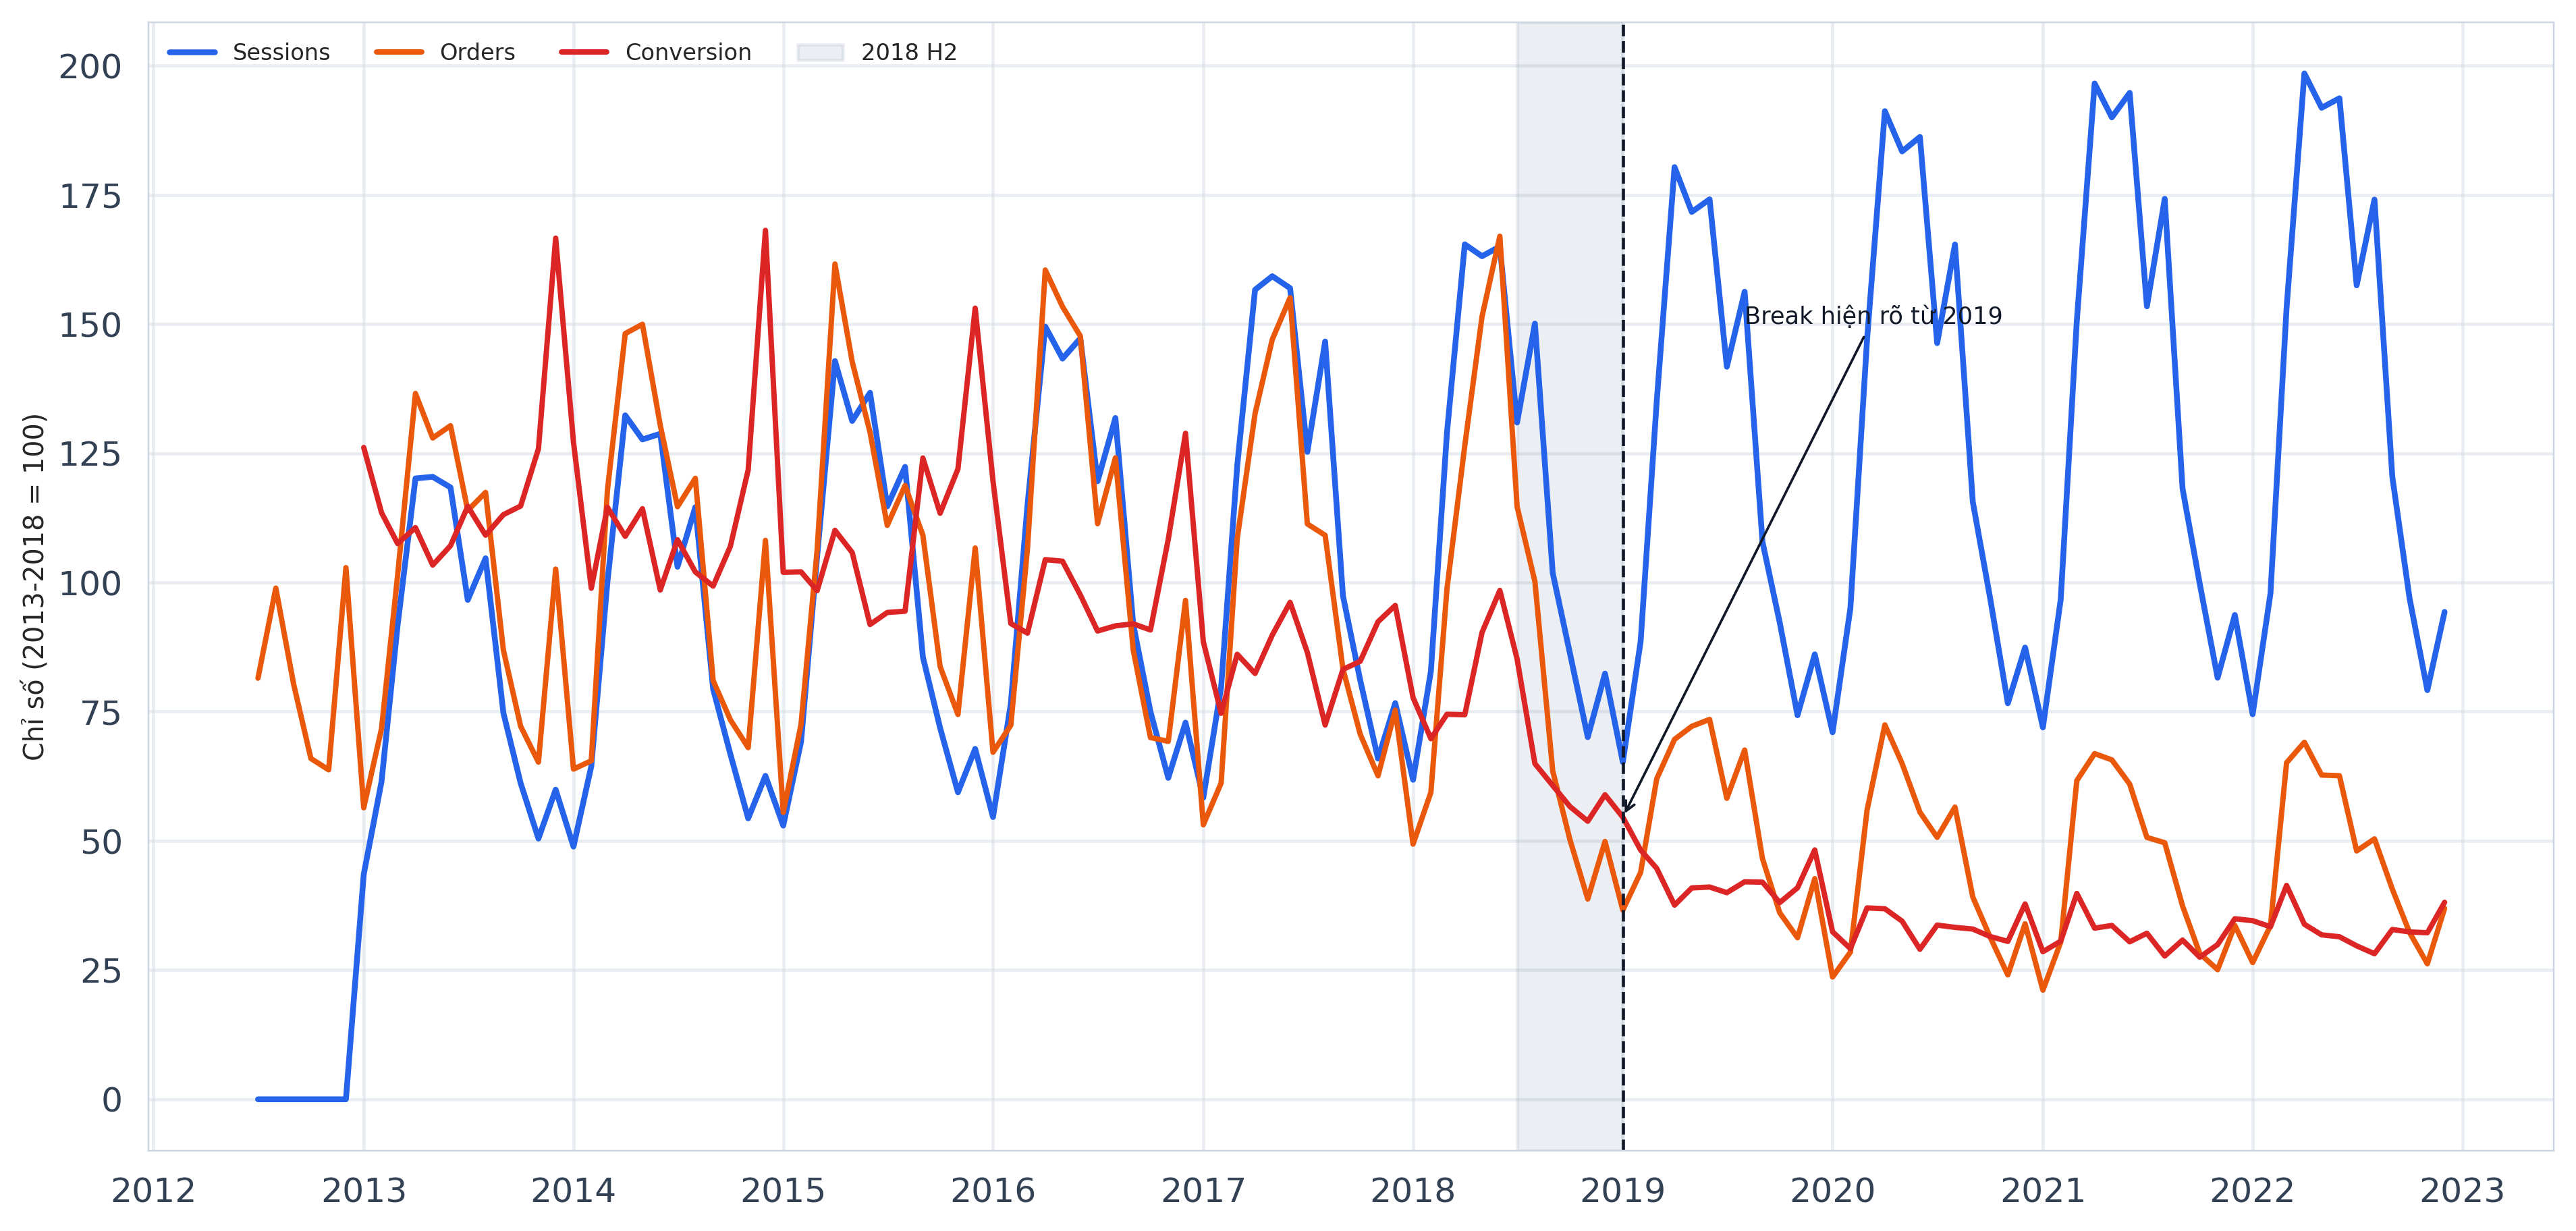
\includegraphics[width=\linewidth]{01_demand_quality_break.png}
\caption{Chất lượng cầu suy giảm sau năm 2019 dù lưu lượng truy cập vẫn tăng.}
\label{fig:demand-break}
\end{figure*}

\subsection{Giảm giá giúp duy trì sản lượng nhưng triệt tiêu giá trị biên}

Hình~\ref{fig:promo-margin} cho thấy ở cả bốn category chính, đơn có giảm giá đều kéo biên lợi nhuận xuống vùng âm, trong khi đơn không giảm giá vẫn giữ được biên dương rõ rệt. Hình~\ref{fig:promo-seasonality} cho thấy cùng một cơ chế lặp lại theo mùa: khuyến mãi giúp giữ số đơn nhưng không tạo ra gross profit tương xứng. Nói cách khác, markdown đang được dùng để bảo vệ volume ngắn hạn và sửa sai cho cơ cấu hàng hóa, thay vì tạo thêm giá trị kinh tế cho mỗi đơn hàng.

\begin{figure*}[t]
\centering
\begin{minipage}[t]{0.49\textwidth}
\centering
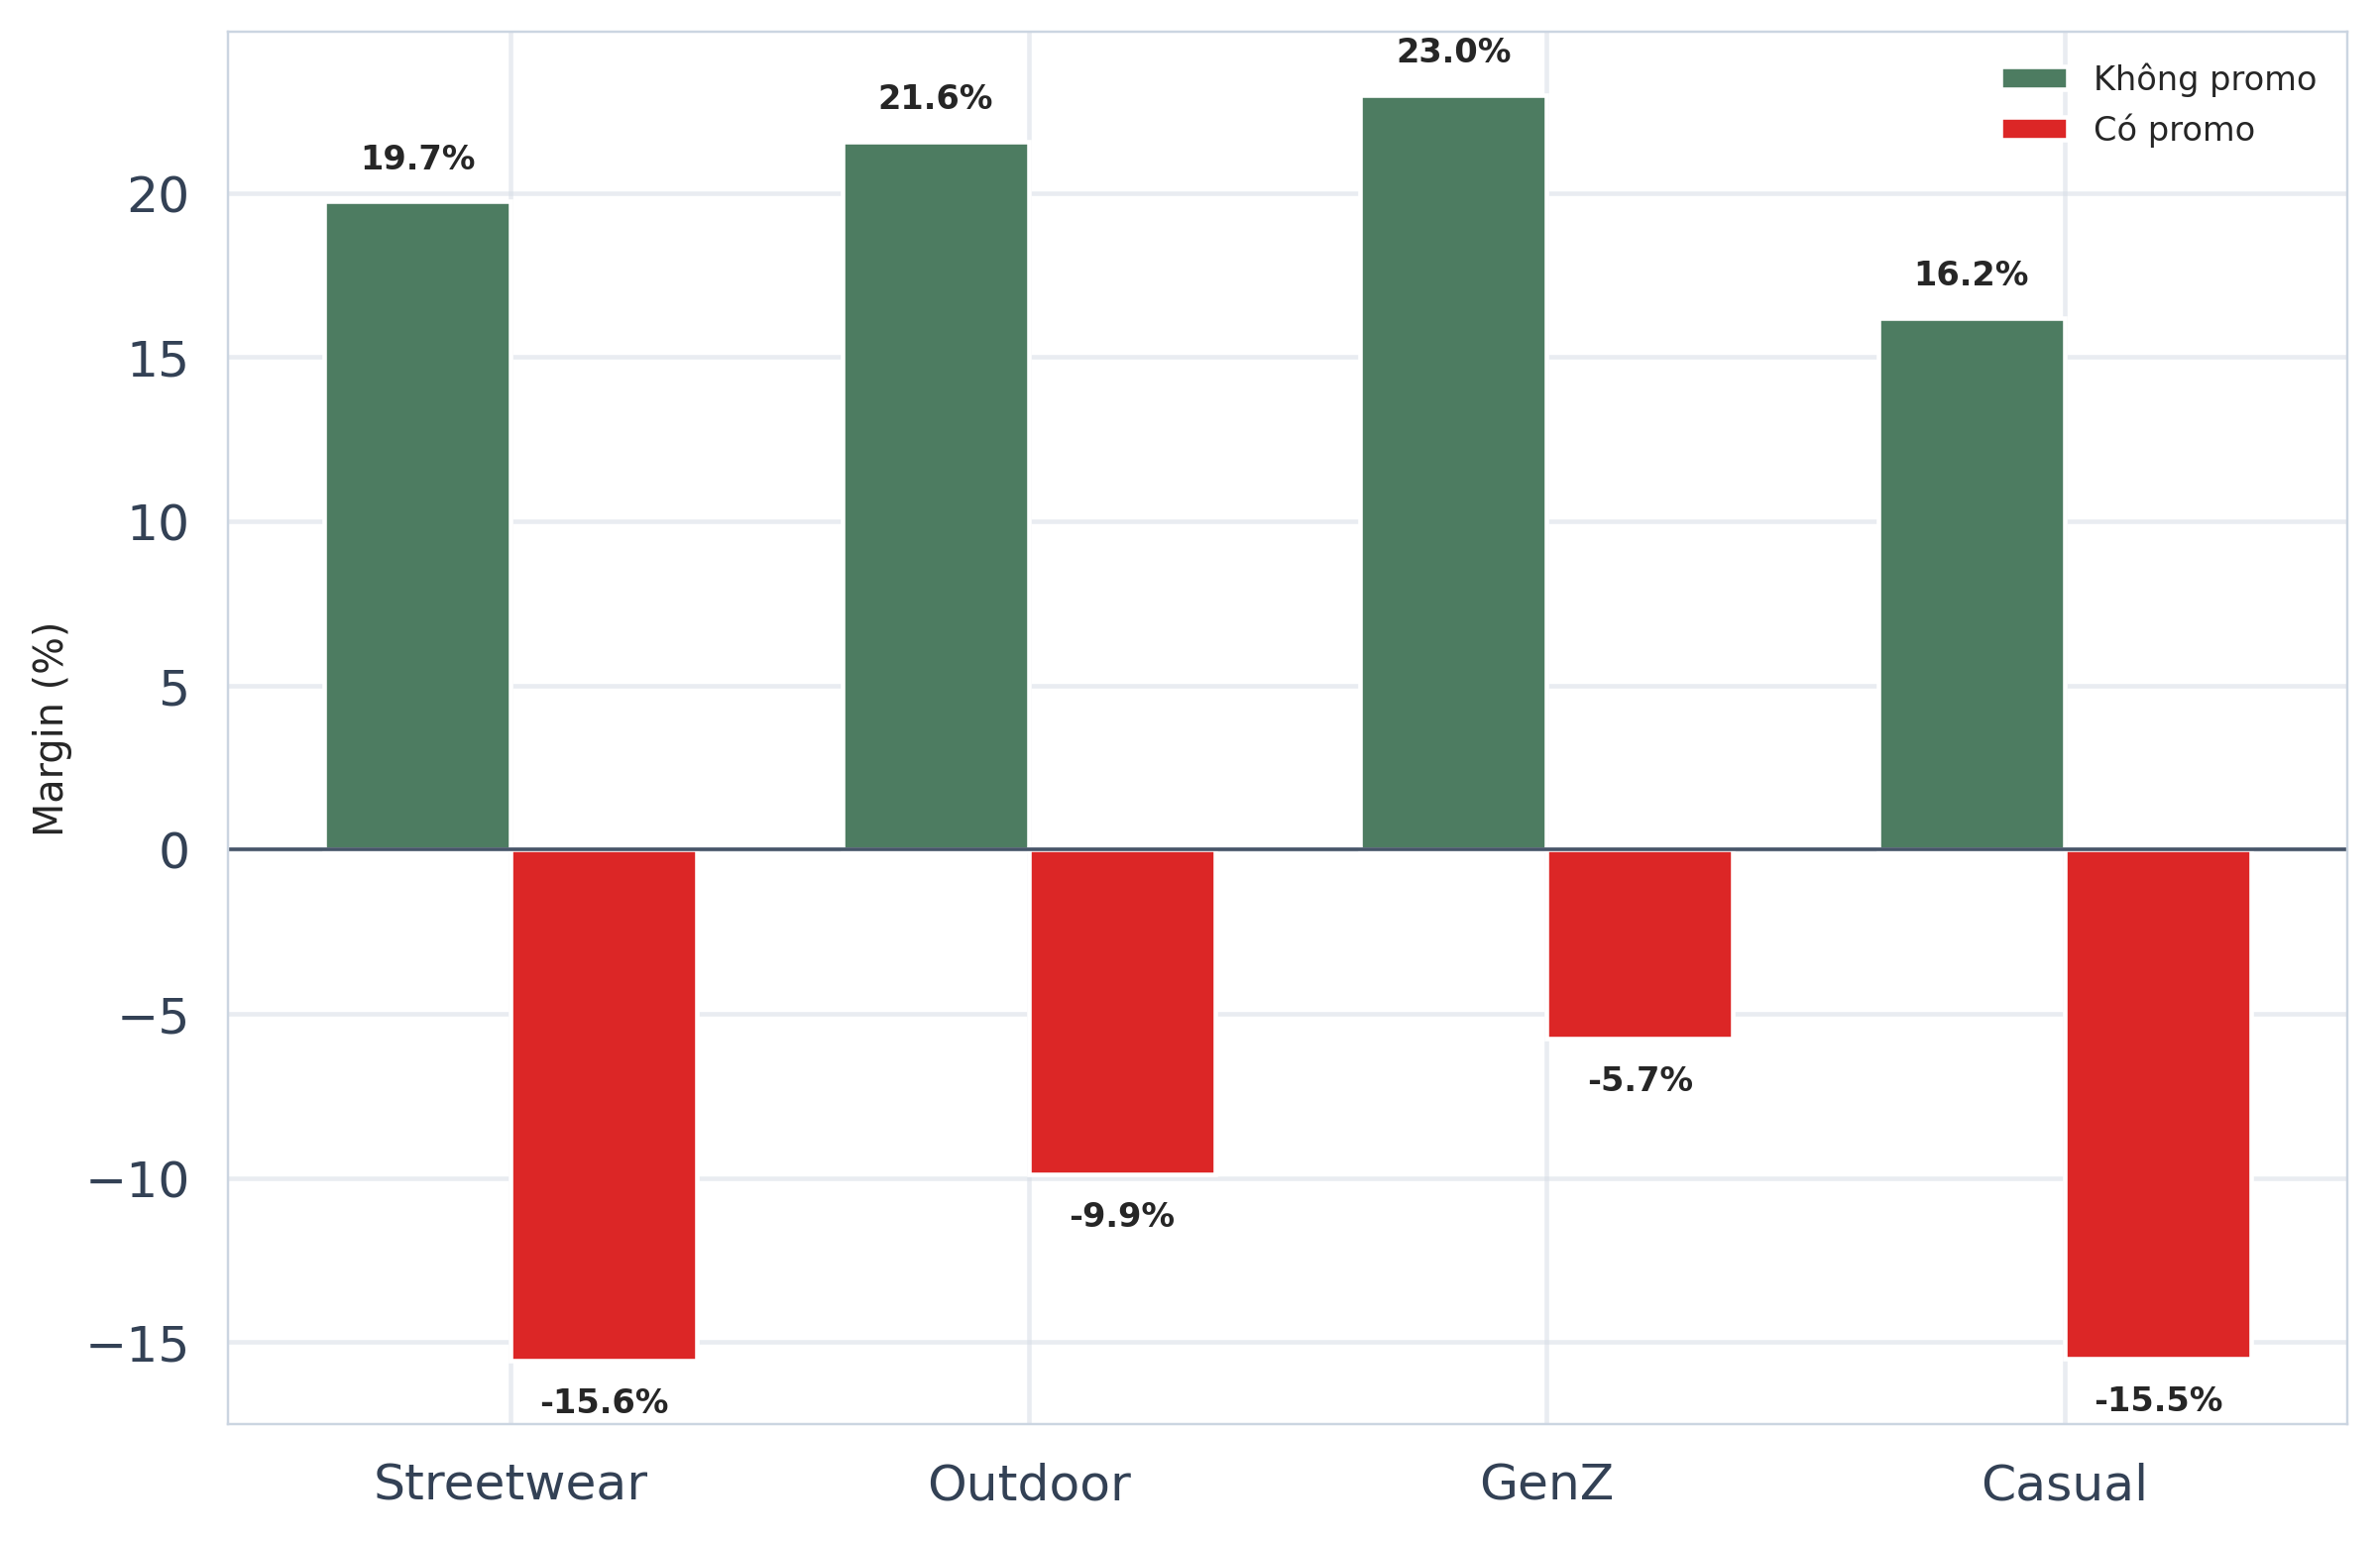
\includegraphics[width=\linewidth]{02_margin_by_category.png}
\captionof{figure}{Margin của đơn giảm giá và không giảm giá theo category.}
\label{fig:promo-margin}
\end{minipage}\hfill
\begin{minipage}[t]{0.49\textwidth}
\centering
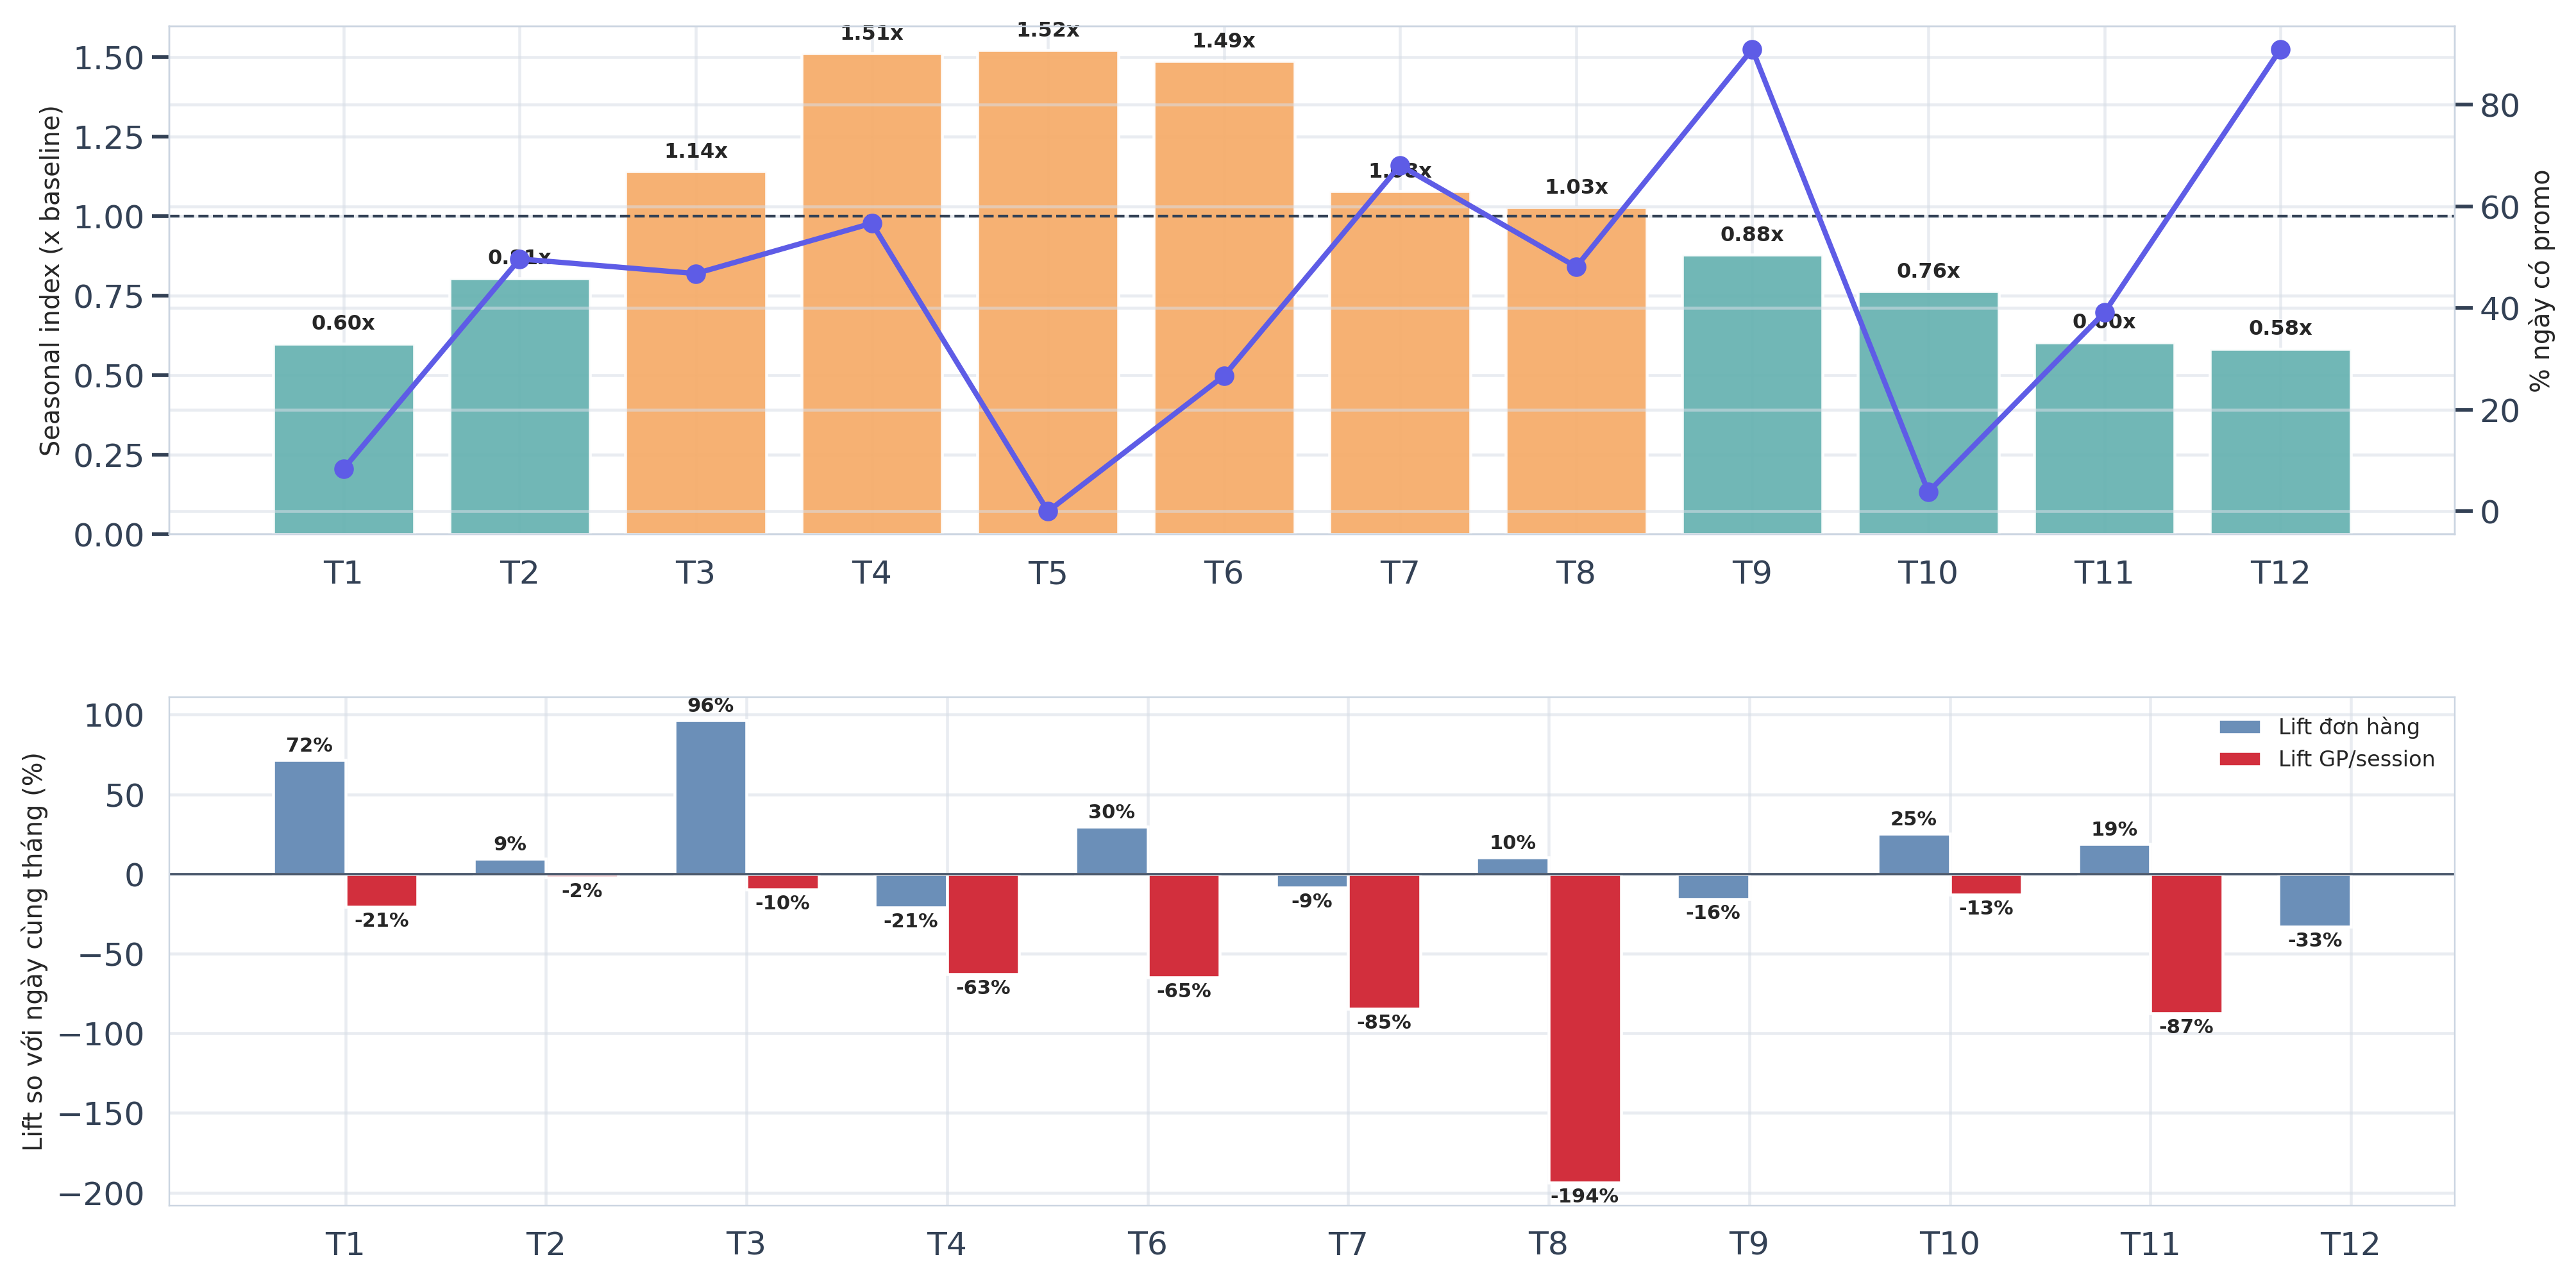
\includegraphics[width=\linewidth]{04_promo_no_incremental_gp.png}
\captionof{figure}{Khuyến mãi đi cùng mùa bán mạnh nhưng không tạo gross profit tương xứng.}
\label{fig:promo-seasonality}
\end{minipage}
\end{figure*}

\subsection{Hàng tồn kho lệch cấu trúc là nguyên nhân chính}
Hình~\ref{fig:root-cause} cho thấy inventory stress đã tăng mạnh từ nửa cuối năm 2018, tức là xuất hiện trước khi doanh thu rơi sâu trong năm 2019. Hình~\ref{fig:inventory-structure} cho thấy các segment lớn nhất đồng thời overstock và stockout, nghĩa là doanh nghiệp vừa giữ quá nhiều hàng chậm quay, vừa thiếu đúng những SKU mà khách hàng cần. Hình~\ref{fig:inventory-flow} cho thấy đây không phải cú sốc ngắn hạn: trong phần lớn chuỗi thời gian, units received thường xuyên cao hơn units sold, trong khi turnover giảm và stockout vẫn cao, cho thấy doanh nghiệp đang vừa nhập dư vừa phục vụ thiếu ở những SKU đúng nhu cầu.


\begin{figure*}[t]
\centering
\begin{minipage}[t]{0.49\textwidth}
\centering
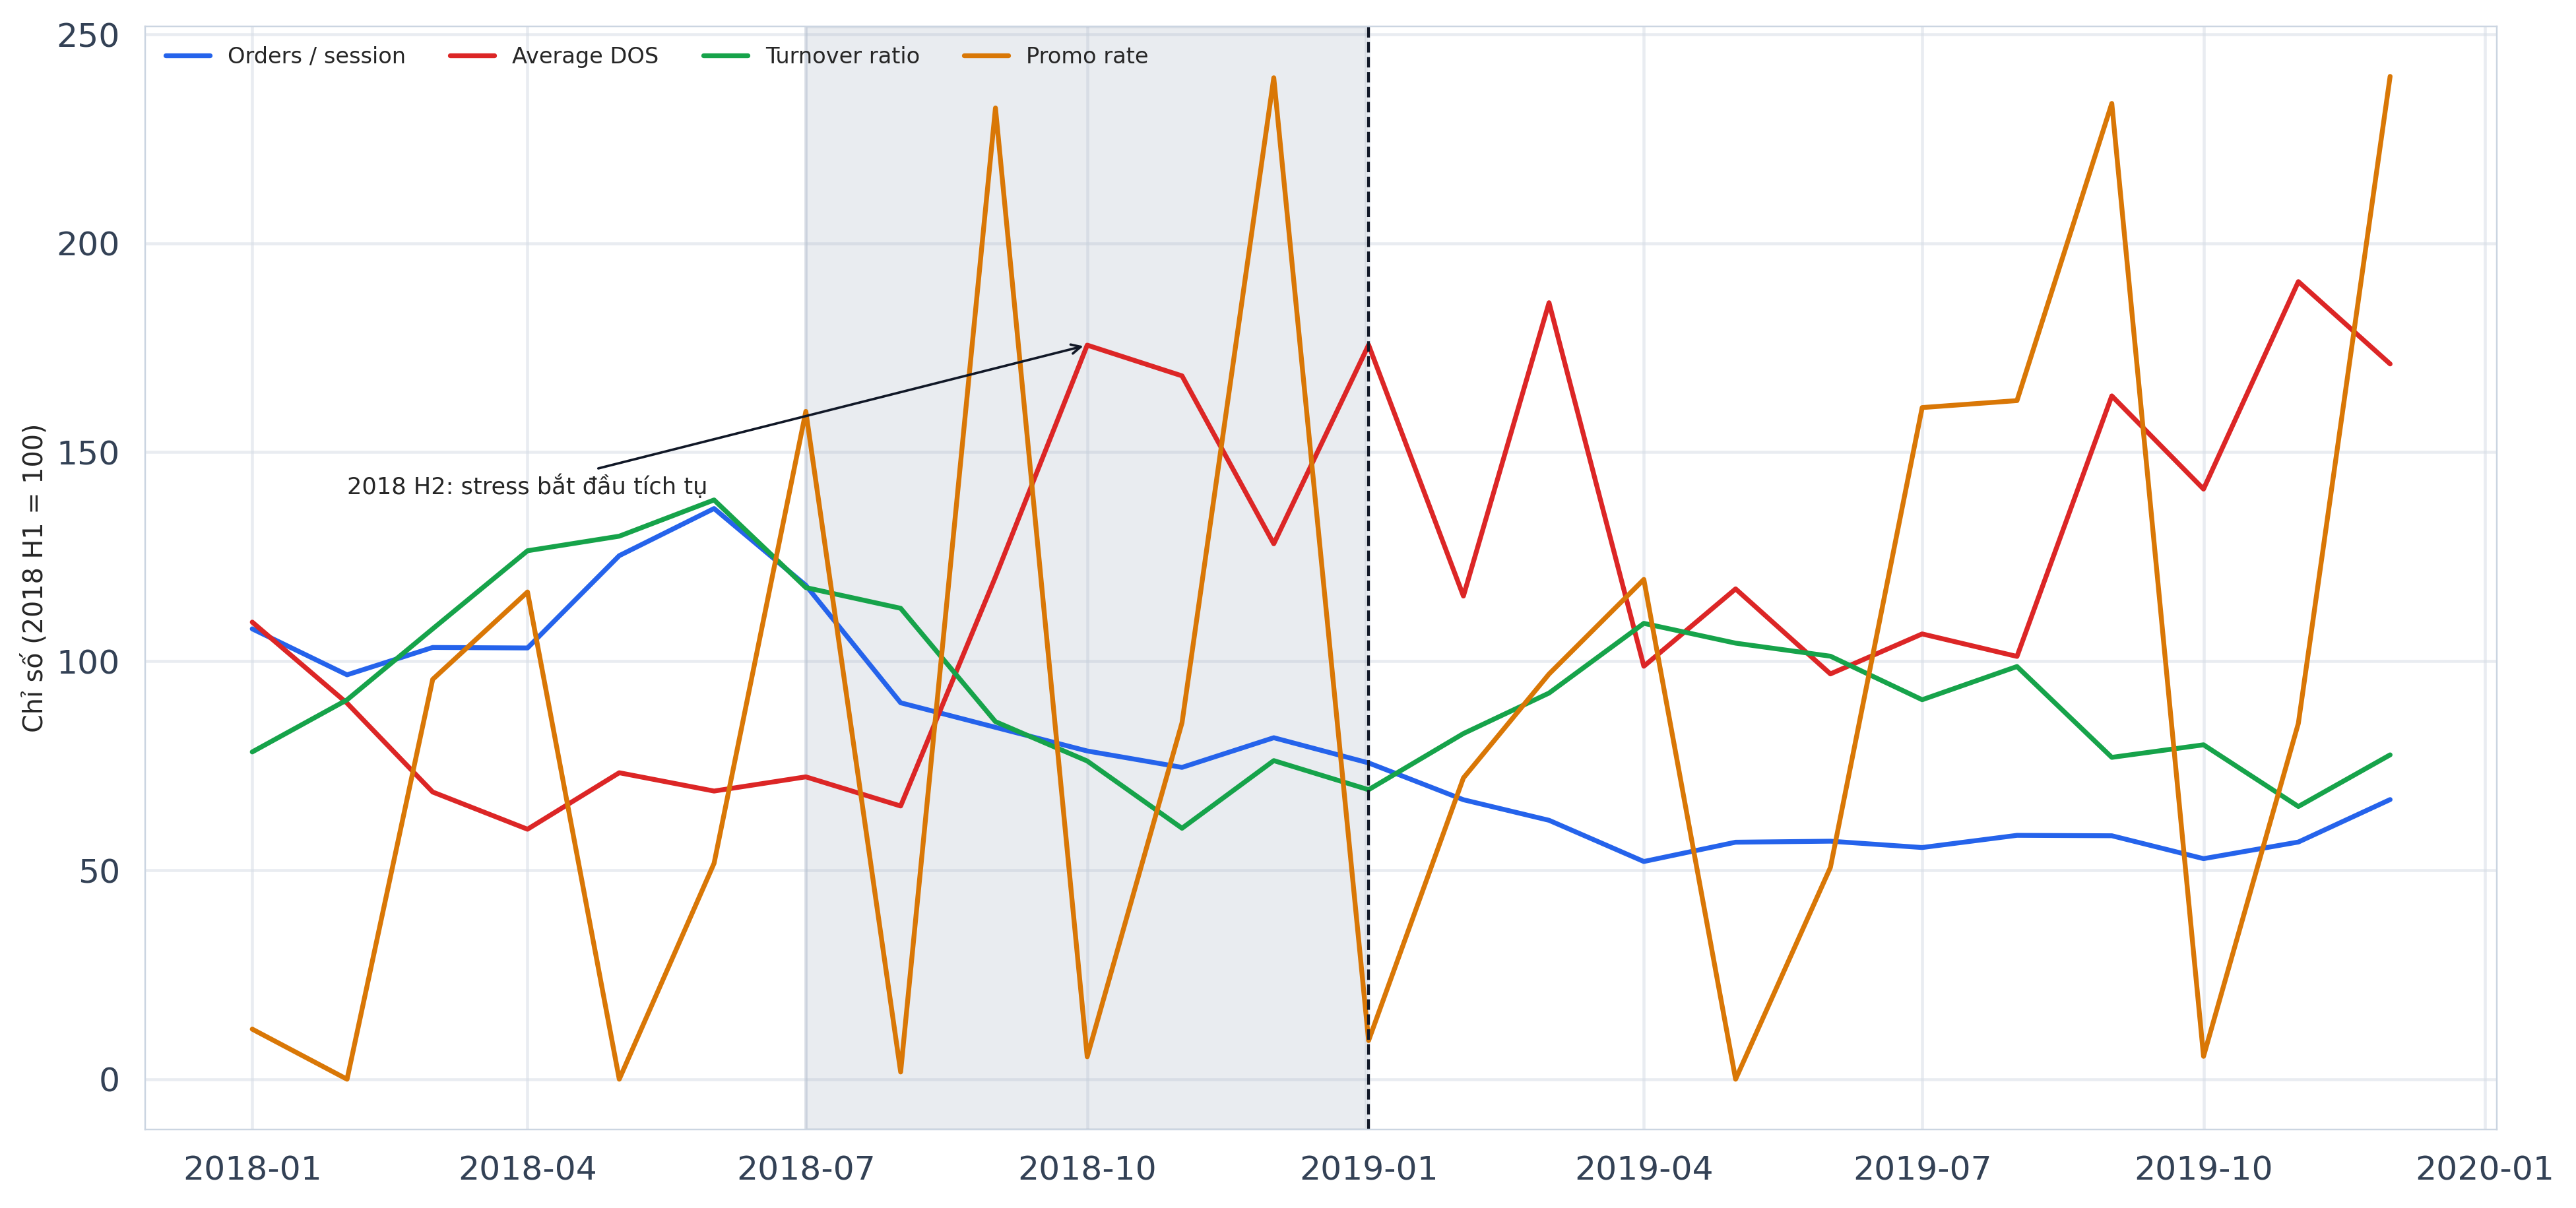
\includegraphics[width=\linewidth]{05_root_cause_2019_inventory_stress.png}
\captionof{figure}{Inventory stress tăng từ 2018 H2 trước khi doanh thu giảm mạnh trong năm 2019.}
\label{fig:root-cause}
\end{minipage}\hfill
\begin{minipage}[t]{0.49\textwidth}
\centering
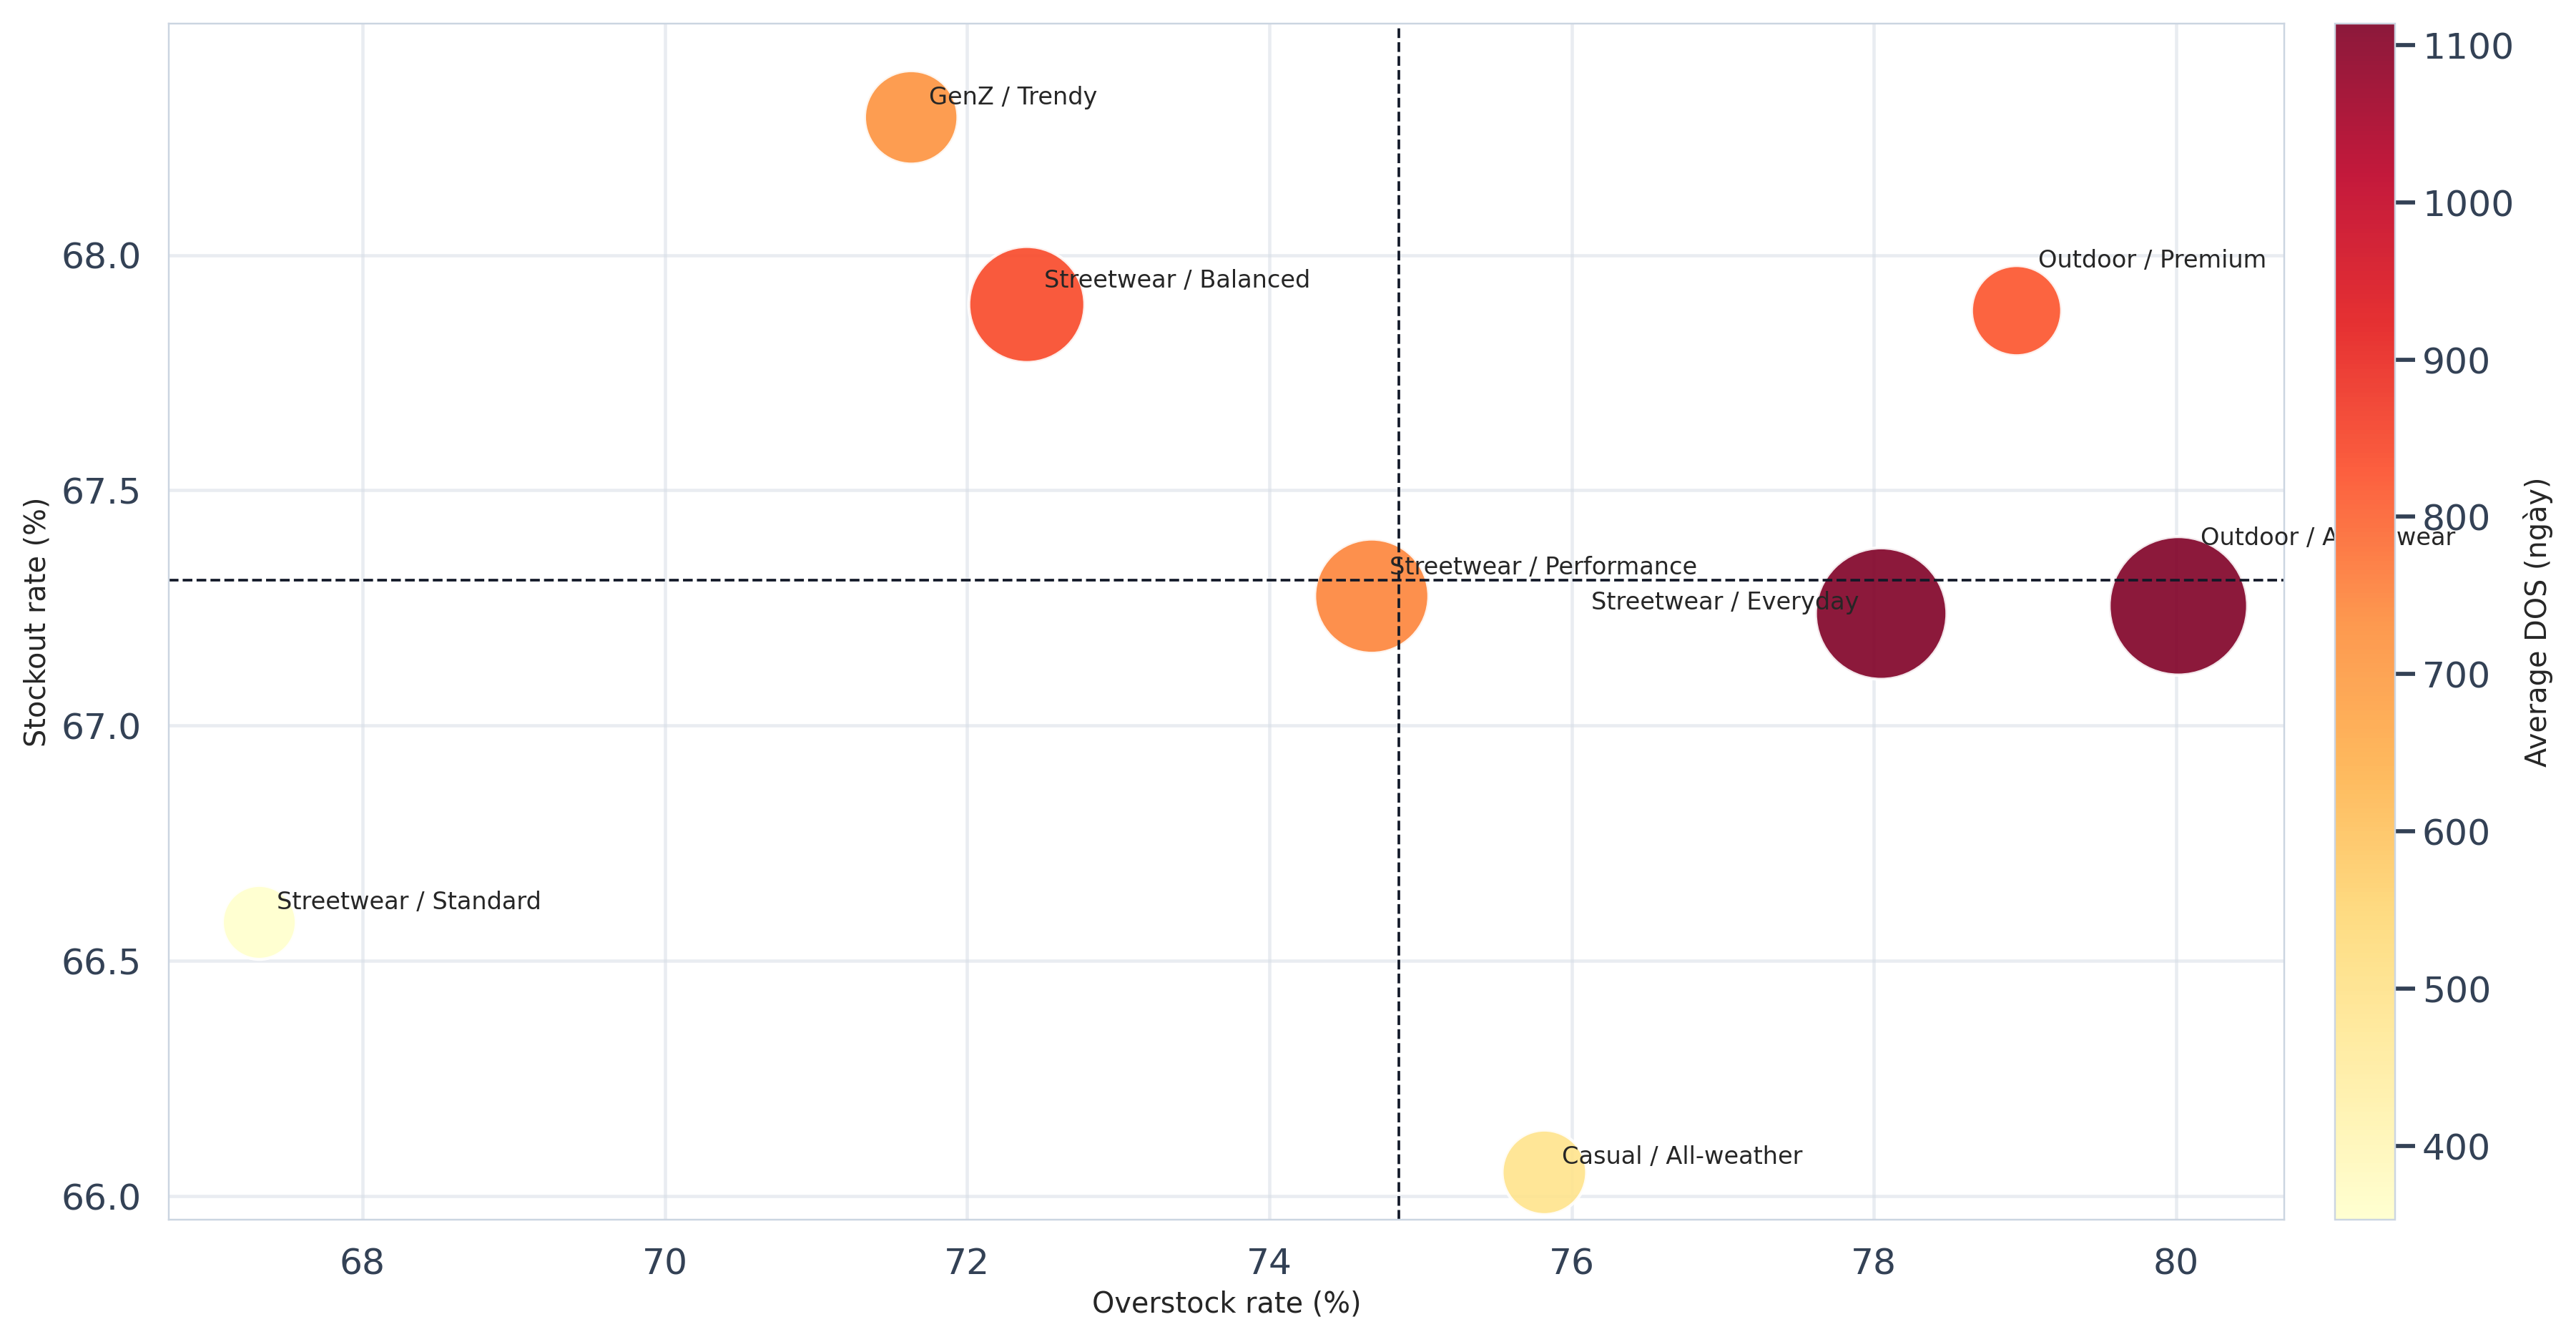
\includegraphics[width=\linewidth]{06_inventory_stress_matrix.png}
\captionof{figure}{Các segment lớn nhất đồng thời overstock và stockout, cho thấy sai lệch ở cơ cấu tồn kho.}
\label{fig:inventory-structure}
\end{minipage}
\end{figure*}

\begin{figure*}[t]
\centering
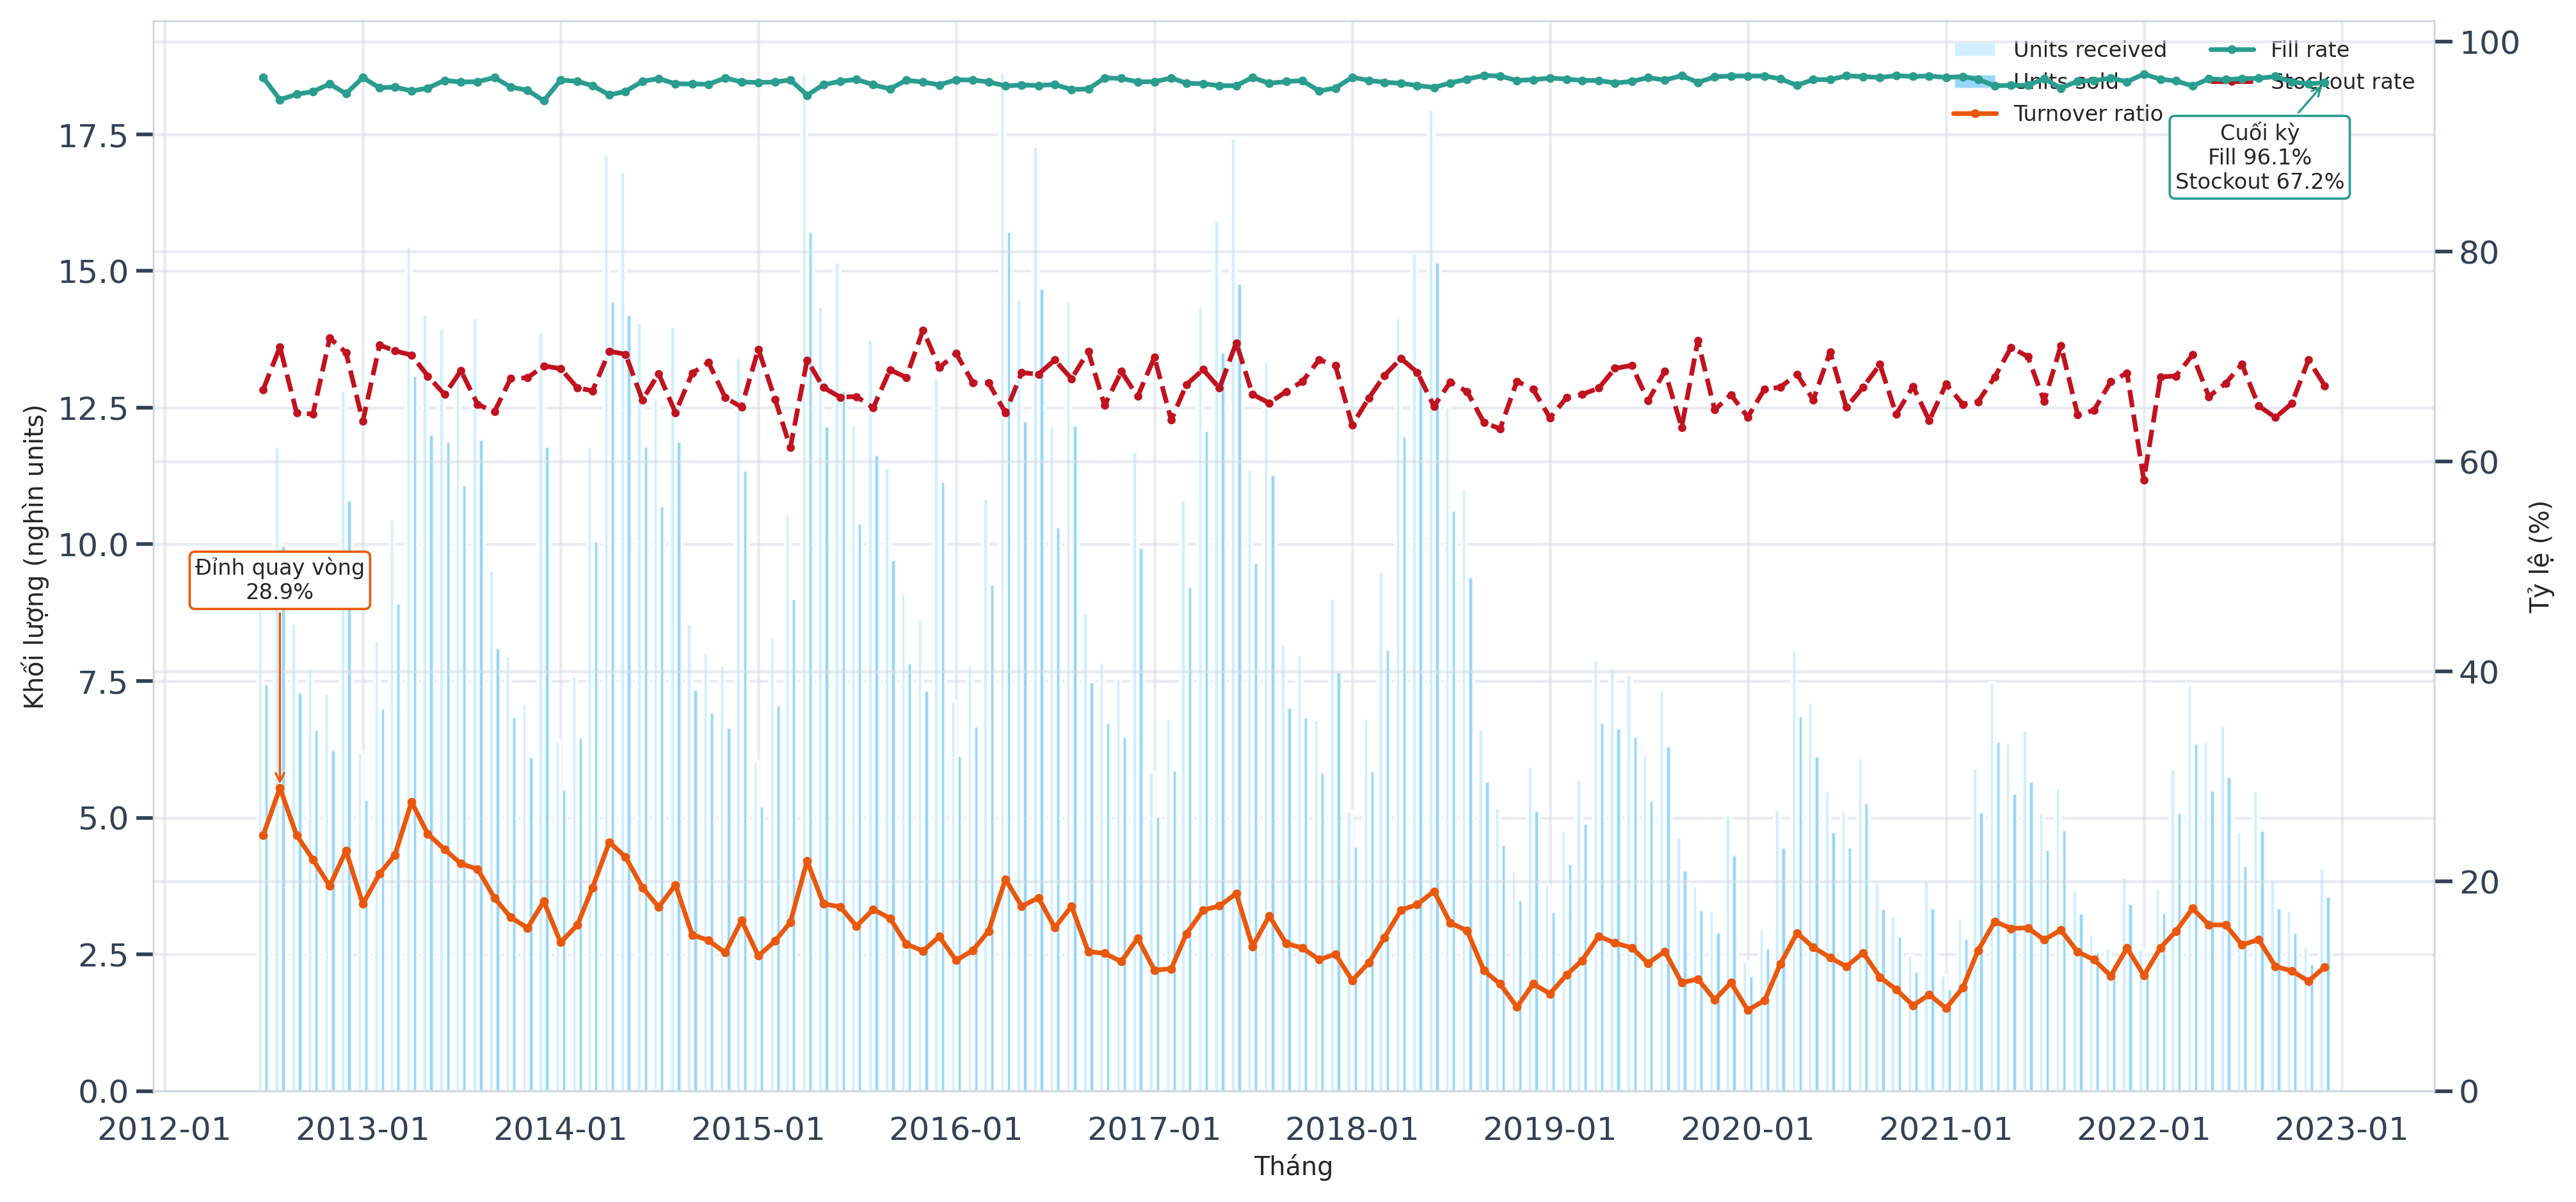
\includegraphics[width=\textwidth]{11_inventory_flow_turnover_service_level.png}
\caption{Dòng hàng hóa, hiệu suất quay vòng và chất lượng phục vụ theo tháng. }
\label{fig:inventory-flow}
\end{figure*}

\subsection{Khuyến mãi đang phủ rộng thay vì đi đúng nhóm khách hàng}
Hình~\ref{fig:rfm-mix} cho thấy doanh thu hiện được giữ bởi một số cụm RFM lớn như Champions, Loyal, Need Attention và At Risk, nhưng tỷ lệ đơn có khuyến mãi giữa các nhóm lại chênh lệch rất ít. Điều này cho thấy doanh nghiệp chưa phân bổ markdown theo giá trị vòng đời hay trạng thái quan hệ của khách hàng, mà đang dùng cùng một công cụ cho các nhóm có vai trò thương mại rất khác nhau.

\begin{figure*}[t]
\centering
\begin{minipage}[t]{0.49\textwidth}
\centering
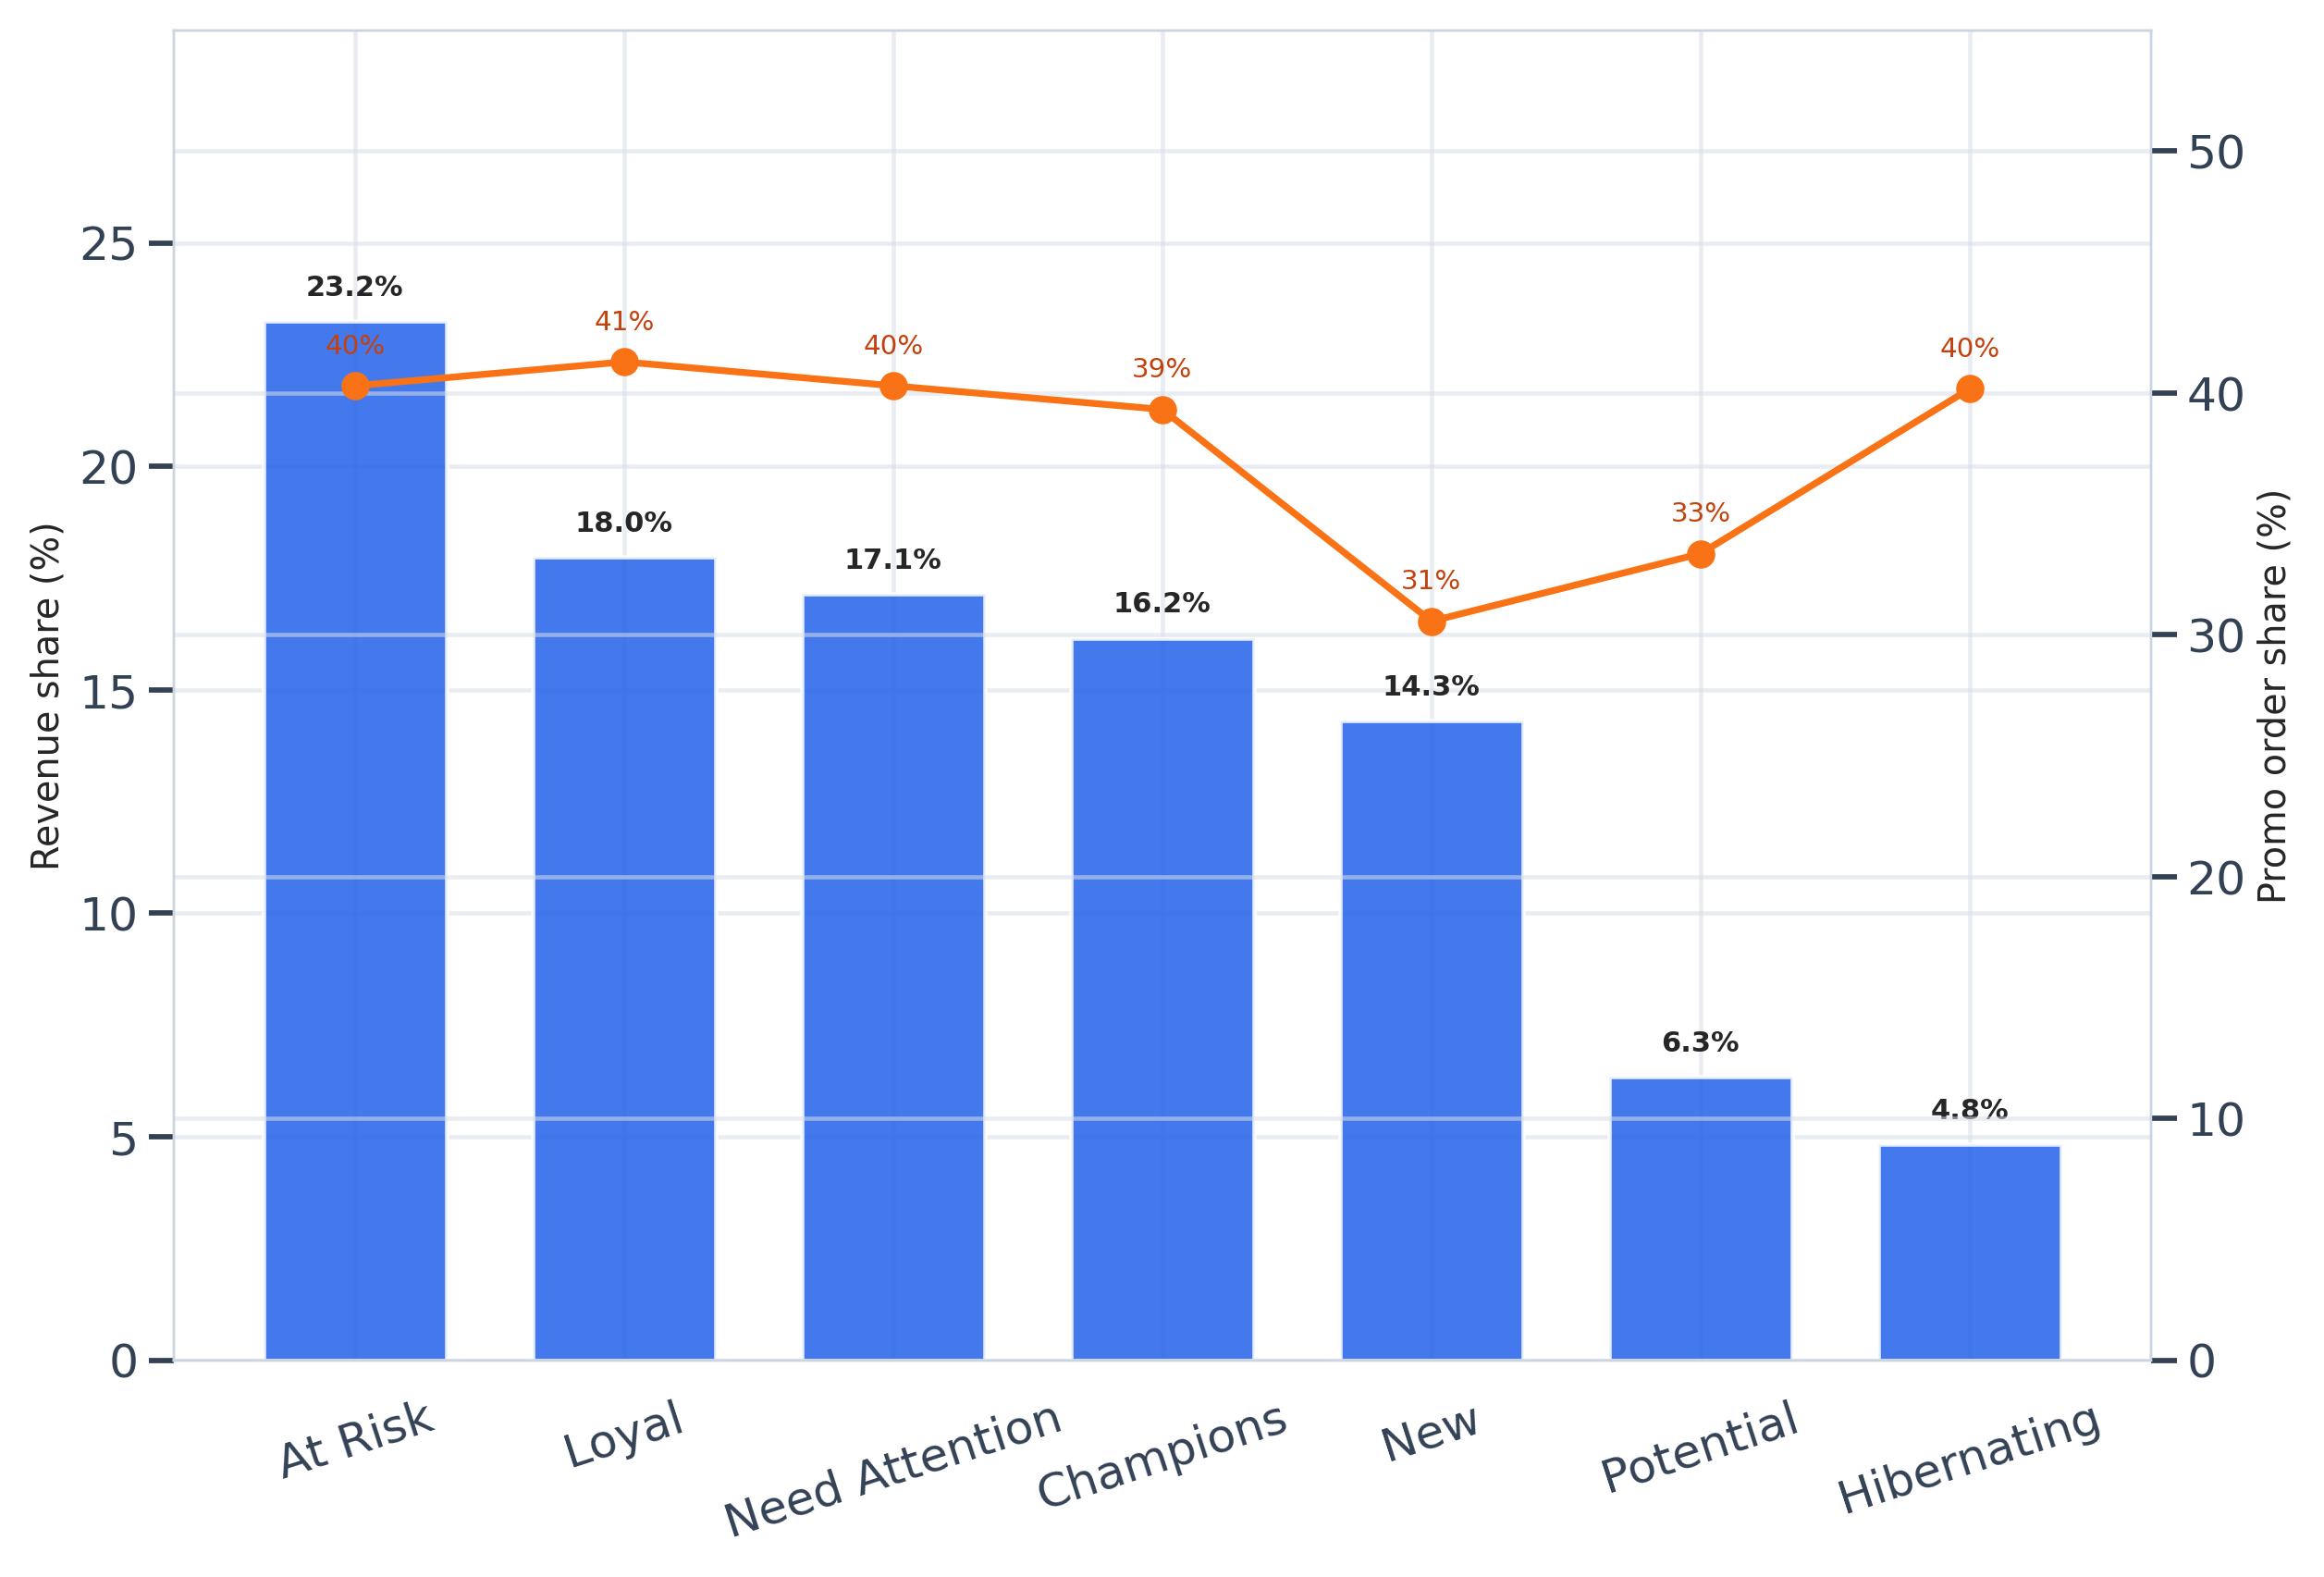
\includegraphics[width=\linewidth]{22_rfm_revenue_mix_promo_share.png}
\captionof{figure}{Doanh thu tập trung ở vài phân khúc RFM lớn, nhưng promo lại khá đều giữa các nhóm.}
\label{fig:rfm-mix}
\end{minipage}\hfill
\begin{minipage}[t]{0.49\textwidth}
\centering
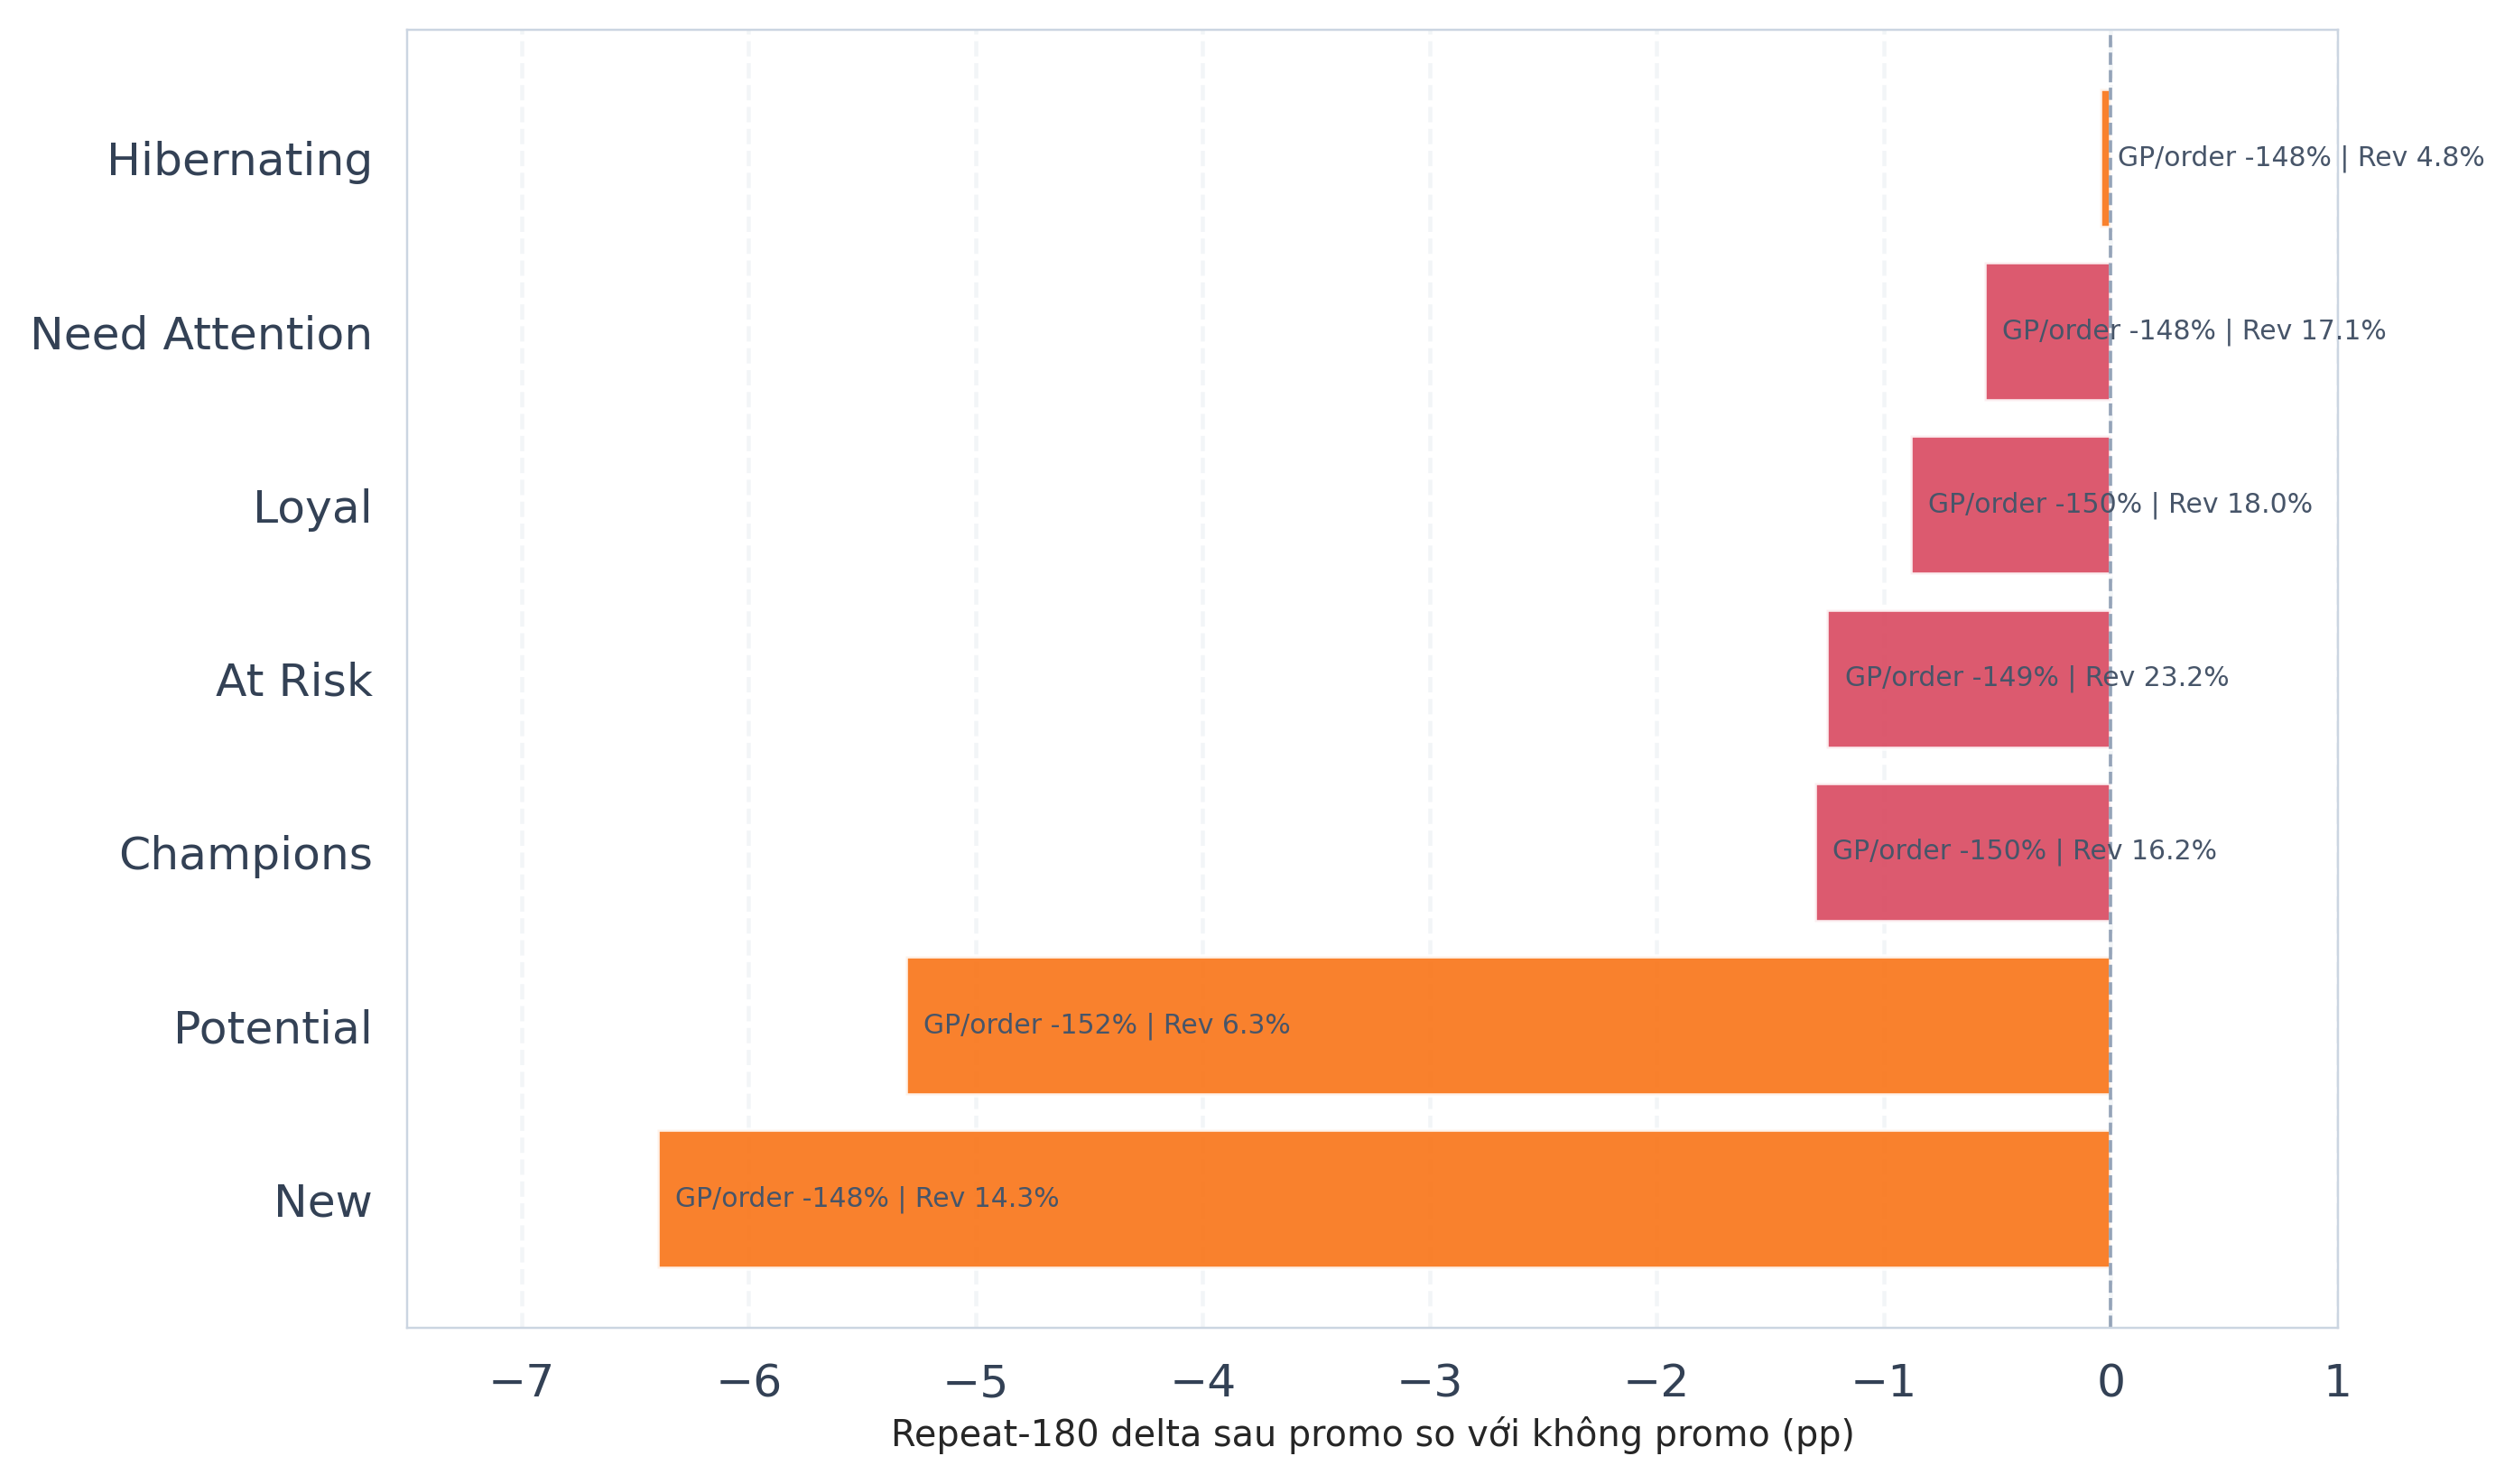
\includegraphics[width=\linewidth]{23_rfm_repeat_delta_after_promo.png}
\captionof{figure}{Promo không cải thiện repeat-180 ở bất kỳ phân khúc RFM nào, trong khi gross profit/ đơn đều giảm mạnh.}
\label{fig:rfm-response}
\end{minipage}
\end{figure*}

Hình~\ref{fig:rfm-response} xác nhận rằng cấu trúc phủ rộng này không tạo ra tín hiệu giữ chân tương xứng với chi phí margin. Ở tất cả các nhóm, repeat-180 sau đơn có khuyến mãi đều thấp hơn hoặc xấp xỉ đơn không khuyến mãi, trong khi gross profit trên mỗi đơn giảm sâu. Kết quả này chưa đủ để khẳng định một causal uplift âm, nhưng đủ để bác bỏ giả thuyết rằng markdown hiện tại đang mua được loyalty với quy mô đáng kể. Champions và Loyal nên được giữ bằng CRM, assortment và trải nghiệm thay vì discount thường xuyên; At Risk và Need Attention phù hợp hơn với các chiến dịch win-back có điều kiện; New và Potential cần onboarding, fit guidance và nội dung sản phẩm tốt hơn trước khi bước vào các vòng giảm giá sâu.

\section{Mô hình dự báo Revenue}
\subsection{Phương pháp và tiêu chuẩn lựa chọn}
\begin{table}[t]
\centering
\small
\caption{Tóm tắt feature groups và kiến trúc của \texttt{meta\_horizon\_nnls}.}
\begin{tabular}{>{\raggedright\arraybackslash}p{0.18\linewidth}>{\raggedright\arraybackslash}p{0.32\linewidth}>{\raggedright\arraybackslash}p{0.38\linewidth}}
\toprule
Nhóm & Thành phần & Vai trò \\
\midrule
Lịch & month, day, dow, doy, days\_to\_month\_end, payday, Fourier terms & Mùa vụ theo tháng, tuần và hiệu ứng cuối tháng \\
Đệ quy doanh thu & rev\_lag\_1, 7, 14, 28; EMA; rolling mean/std & Bám nhịp doanh thu ngắn hạn và quán tính mua lặp \\
Thành phần thương mại & orders, AOV, orders $\times$ AOV & Ổn định phần xa của horizon và hạn chế drift \\
Regime & post-2019 flag, event windows, odd-year August, recent user growth & Hấp thụ đứt gãy theo giai đoạn và anomaly theo mùa \\
Meta-layer & OOF NNLS theo bucket early, mid, late & Trộn specialist bằng trọng số không âm, dễ giải thích \\
\bottomrule
\end{tabular}
\end{table}

Mục tiêu là dự báo Revenue hằng ngày trên horizon dài với sai số phụ thuộc vị trí kỳ dự báo. Final line \texttt{meta_horizon_nnls} là meta-ensemble với trọng số không âm theo ba bucket: early, mid, late. Base learners gồm baseline seasonality, recursive revenue head, decomposition orders $\times$ AOV và revenue regime specialist. Các head học bằng gradient-boosted trees trên dự báo out-of-fold; meta-layer dùng NNLS để trộn, giữ tính minh bạch.

Candidate được xây từ dữ liệu chính thức, đánh giá bằng rolling out-of-fold và đối chiếu public để loại cấu hình kém ổn định. \texttt{meta_horizon_ridge} tốt nhất internal, còn \texttt{meta_horizon_nnls} mạnh và ổn định nhất trên public nên được chọn.

\subsection{Kết quả và diễn giải mô hình}
\texttt{meta_horizon_nnls} thay đổi trọng số theo horizon: early $\sim$76.5\% recursive và 23.5\% component; sang mid/late, trọng số dịch dần về component, recursive vẫn làm nền. Ngắn hạn bị chi phối bởi quán tính; dài hạn dựa nhiều vào orders $\times$ AOV.

SHAP xác nhận rằng recursive quan trọng với \texttt{rev_lag_1}, \texttt{rev_lag_7}, \texttt{rev_ema_3}, \texttt{days_to_month_end}, \texttt{day_of_month}, \texttt{recent_user_growth}; regime nổi bật với \texttt{year}, \texttt{recent_user_growth}, \texttt{is_post_2019}, \texttt{day_of_week}, \texttt{event_service_interact}, \texttt{is_odd_year_august}. Forecast nhất quán với Part 2, chỉ kéo dài cơ chế này về phía trước.

\section{Hàm ý điều hành}
Hình~\ref{fig:action-tradeoff} cho thấy con đường hợp lý không phải là giữ mọi đơn hàng bằng mọi giá, mà là chấp nhận cắt phần volume kém chất lượng để phục hồi khả năng sinh doanh thu lành mạnh. Thứ tự hành động vì vậy phải đi theo đúng chuỗi thất thoát giá trị đã được chỉ ra trong dữ liệu: siết markdown sâu, làm sạch core inventory ở các segment vừa overstock vừa stockout, rồi mới xử lý ma sát ở size guidance, mô tả sản phẩm và checkout. Nếu đảo ngược thứ tự này, doanh nghiệp sẽ tiếp tục mua thêm demand cho một hệ thống vẫn chưa sửa được các điểm mất giá trị cốt lõi.

\begin{figure*}[t]
\centering
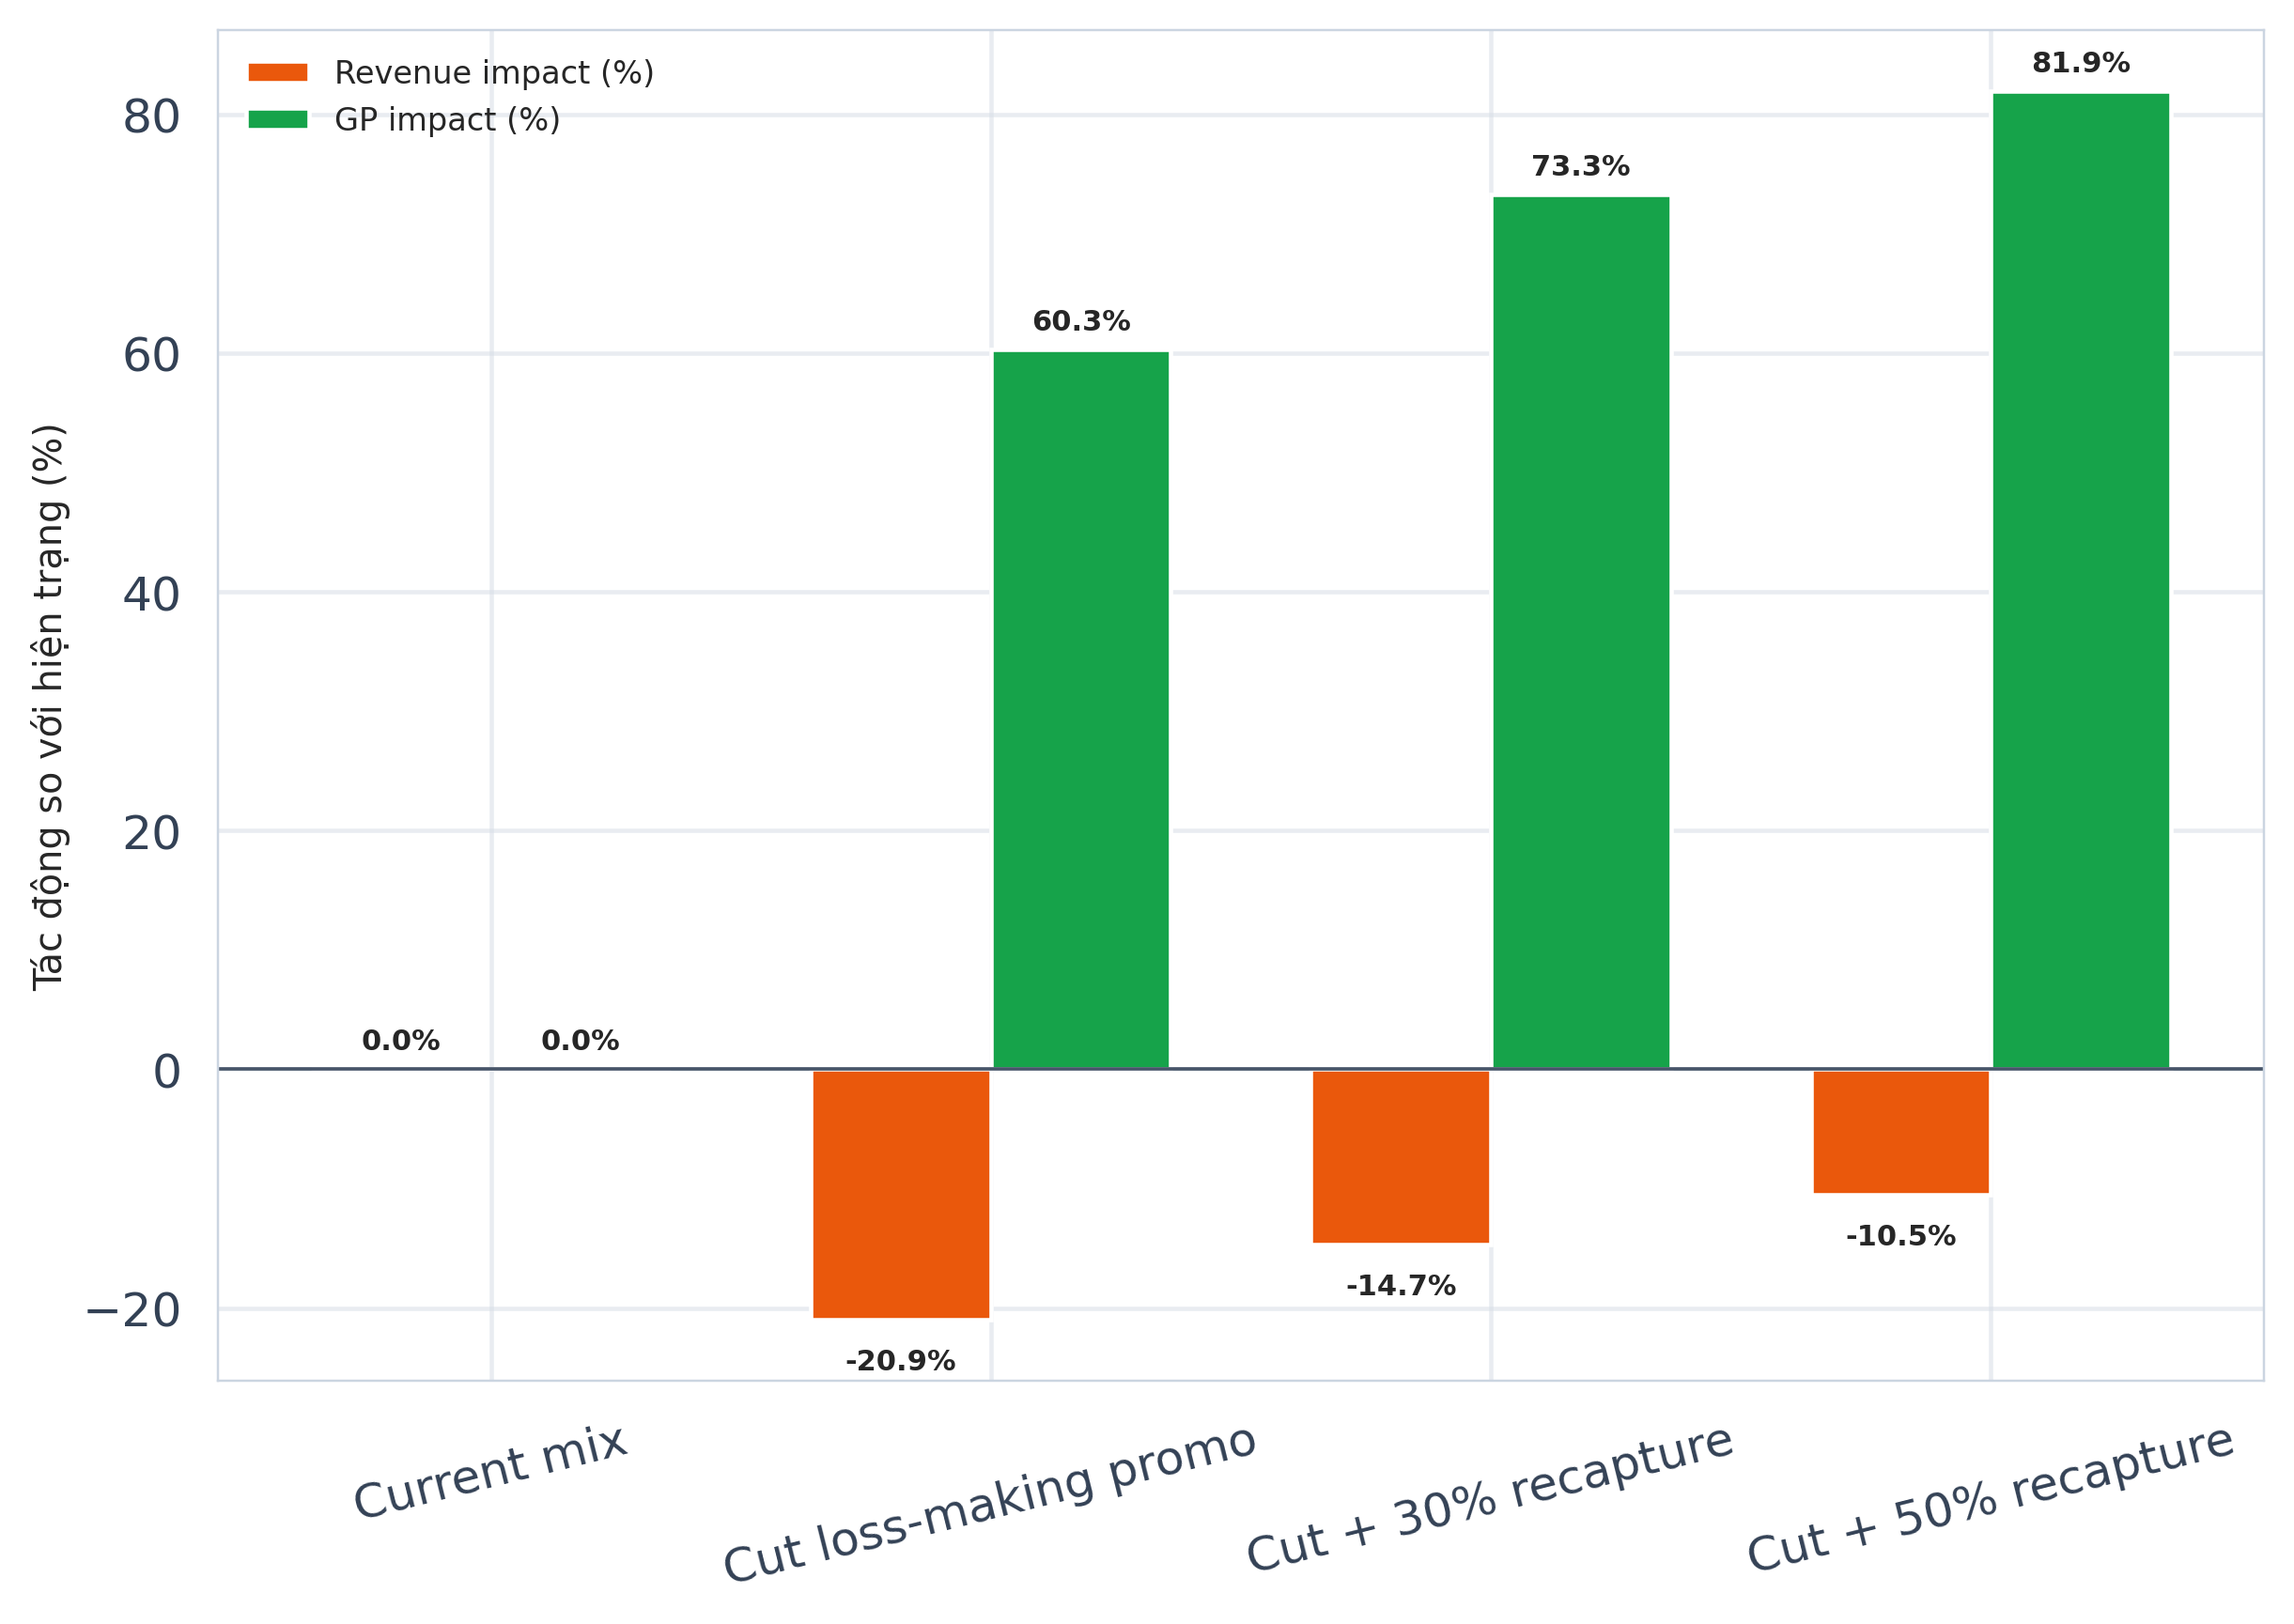
\includegraphics[width=\textwidth]{20_action_tradeoff_scenarios.png}
\caption{Trade-off giữa doanh thu và gross profit dưới các kịch bản hành động. Kịch bản hợp lý không phải là giữ mọi đơn hàng bằng mọi giá, mà là chấp nhận cắt phần volume phá giá trị để phục hồi gross profit và vòng quay vốn.}
\label{fig:action-tradeoff}
\end{figure*}

\section{Kết luận}
Bộ dữ liệu này cho thấy doanh nghiệp không suy giảm vì thiếu nhu cầu tuyệt đối, mà vì liên tục làm rò rỉ giá trị trong quá trình biến nhu cầu thành doanh thu thực chất. Điểm gãy xuất hiện trước hết ở conversion, sau đó lan sang economics của đơn hàng và tích tụ thành áp lực tồn kho. Khi mô hình dự báo Revenue được xây trên đúng các driver đó, forecasting trở thành bước kiểm định cuối cùng cho toàn bộ lập luận kinh doanh.

\clearpage
\appendix
\section{Phụ lục diễn giải mô hình}
Các bảng SHAP và thống kê ổn định theo fold được xuất tại thư mục appendix của repo. Trong bản phụ lục trực quan, chúng tôi giữ ba nhóm hình chính: phân bổ trọng số theo horizon, tổng hợp SHAP cho revenue specialist và độ ổn định của feature importance theo fold.

\begin{figure*}[p]
\centering
\centering
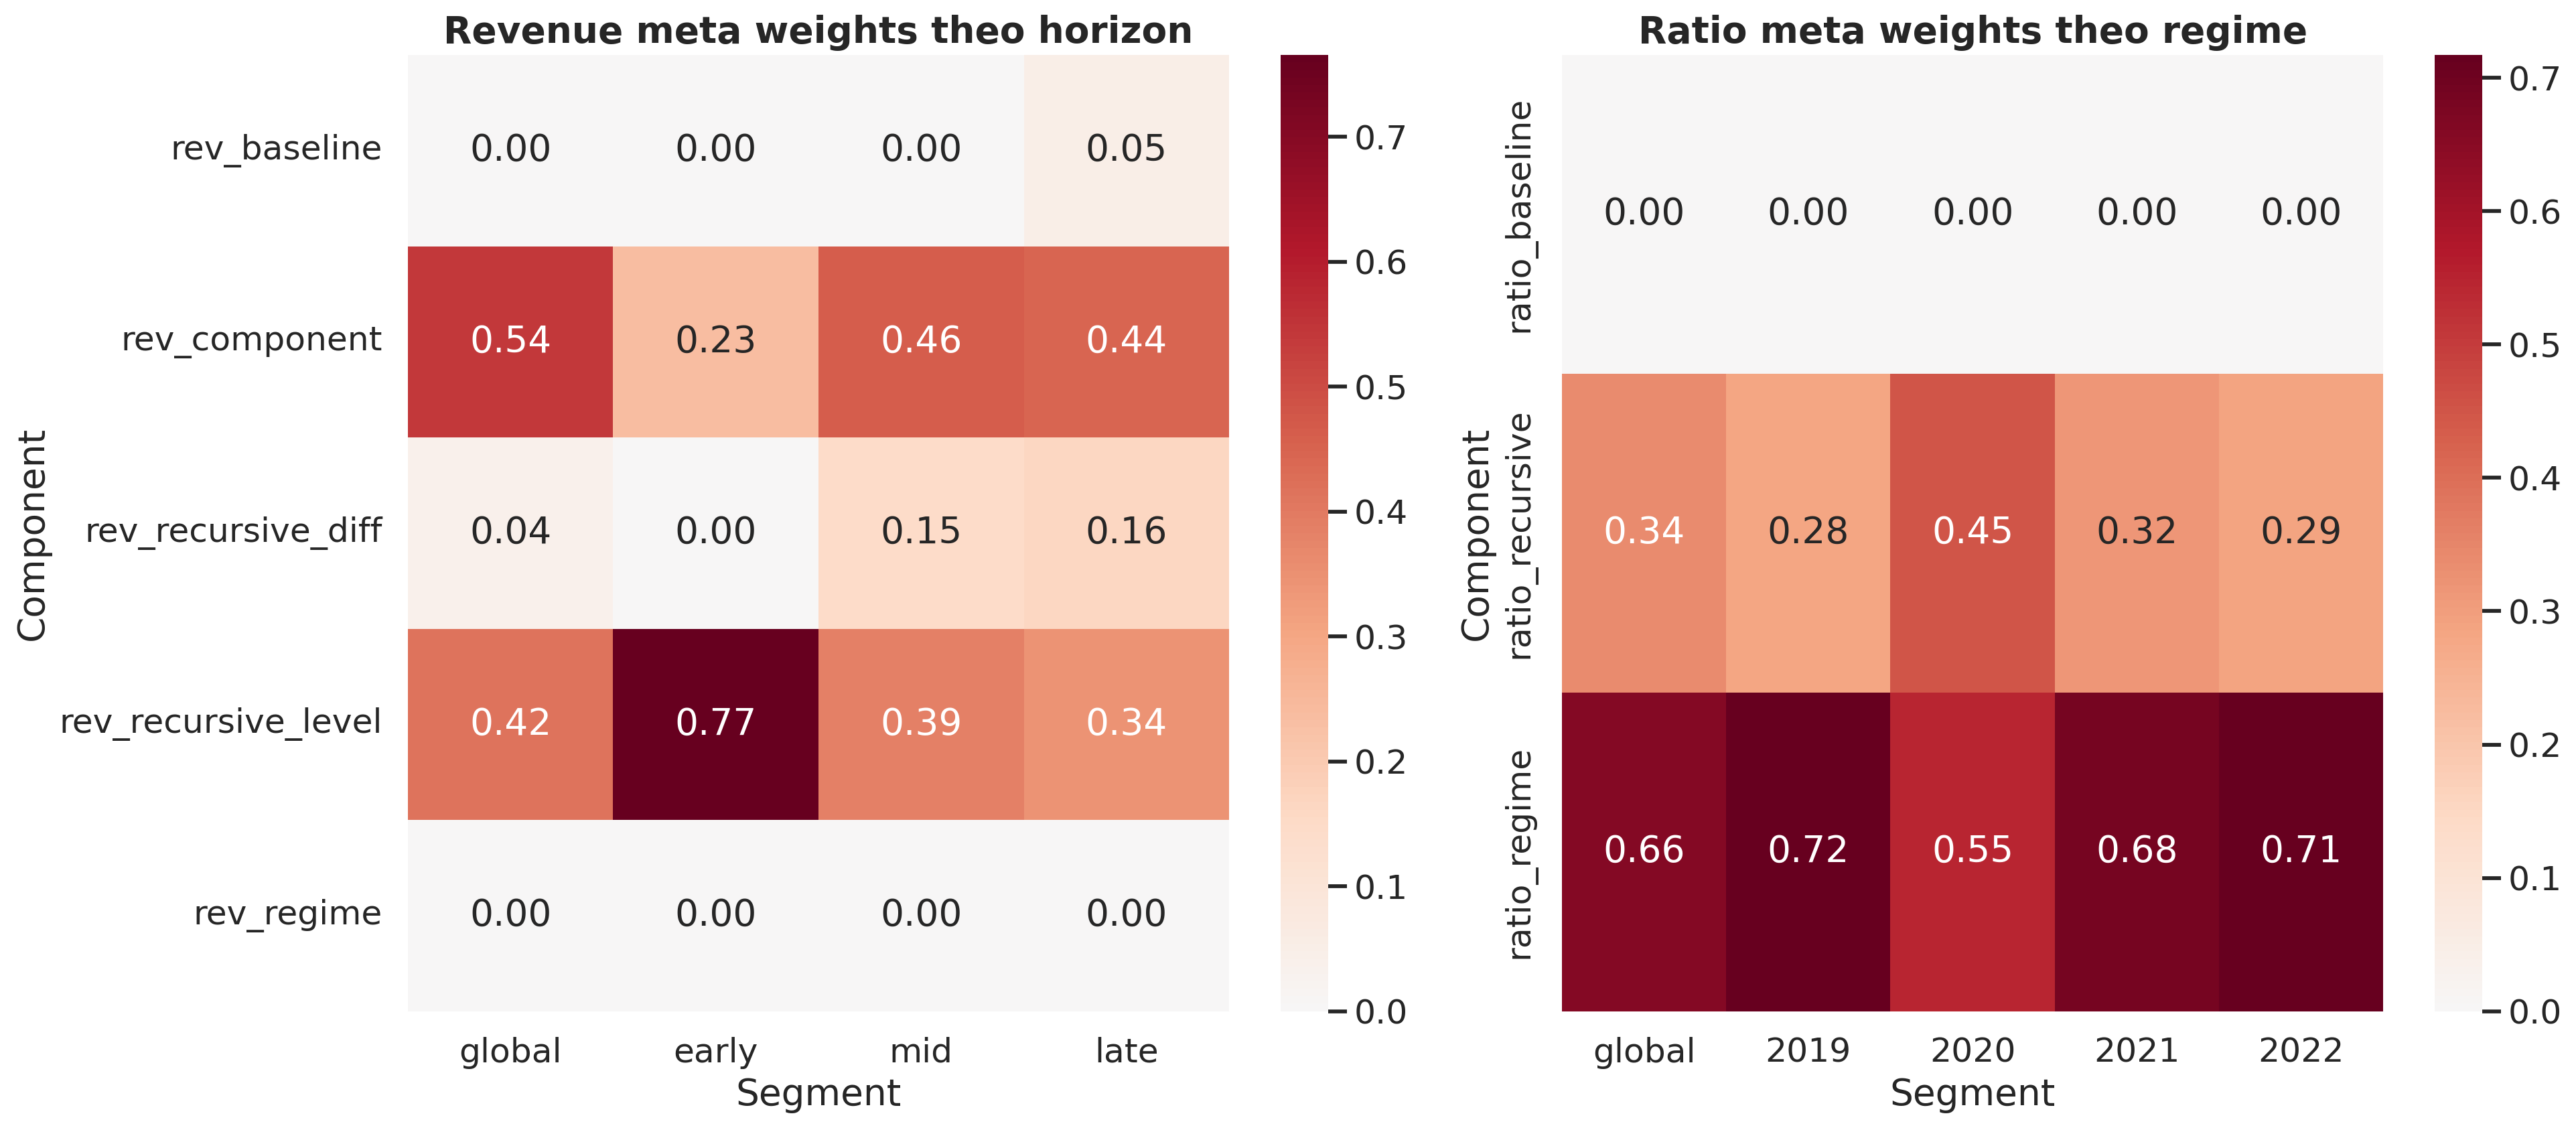
\includegraphics[width=\linewidth]{21_meta_horizon_weight_heatmap.png}
\captionof{figure}{Phân bổ trọng số của meta-layer theo từng bucket horizon.}
\label{fig:appendix-weights}
\end{figure*}

\begin{figure*}[p]
\centering
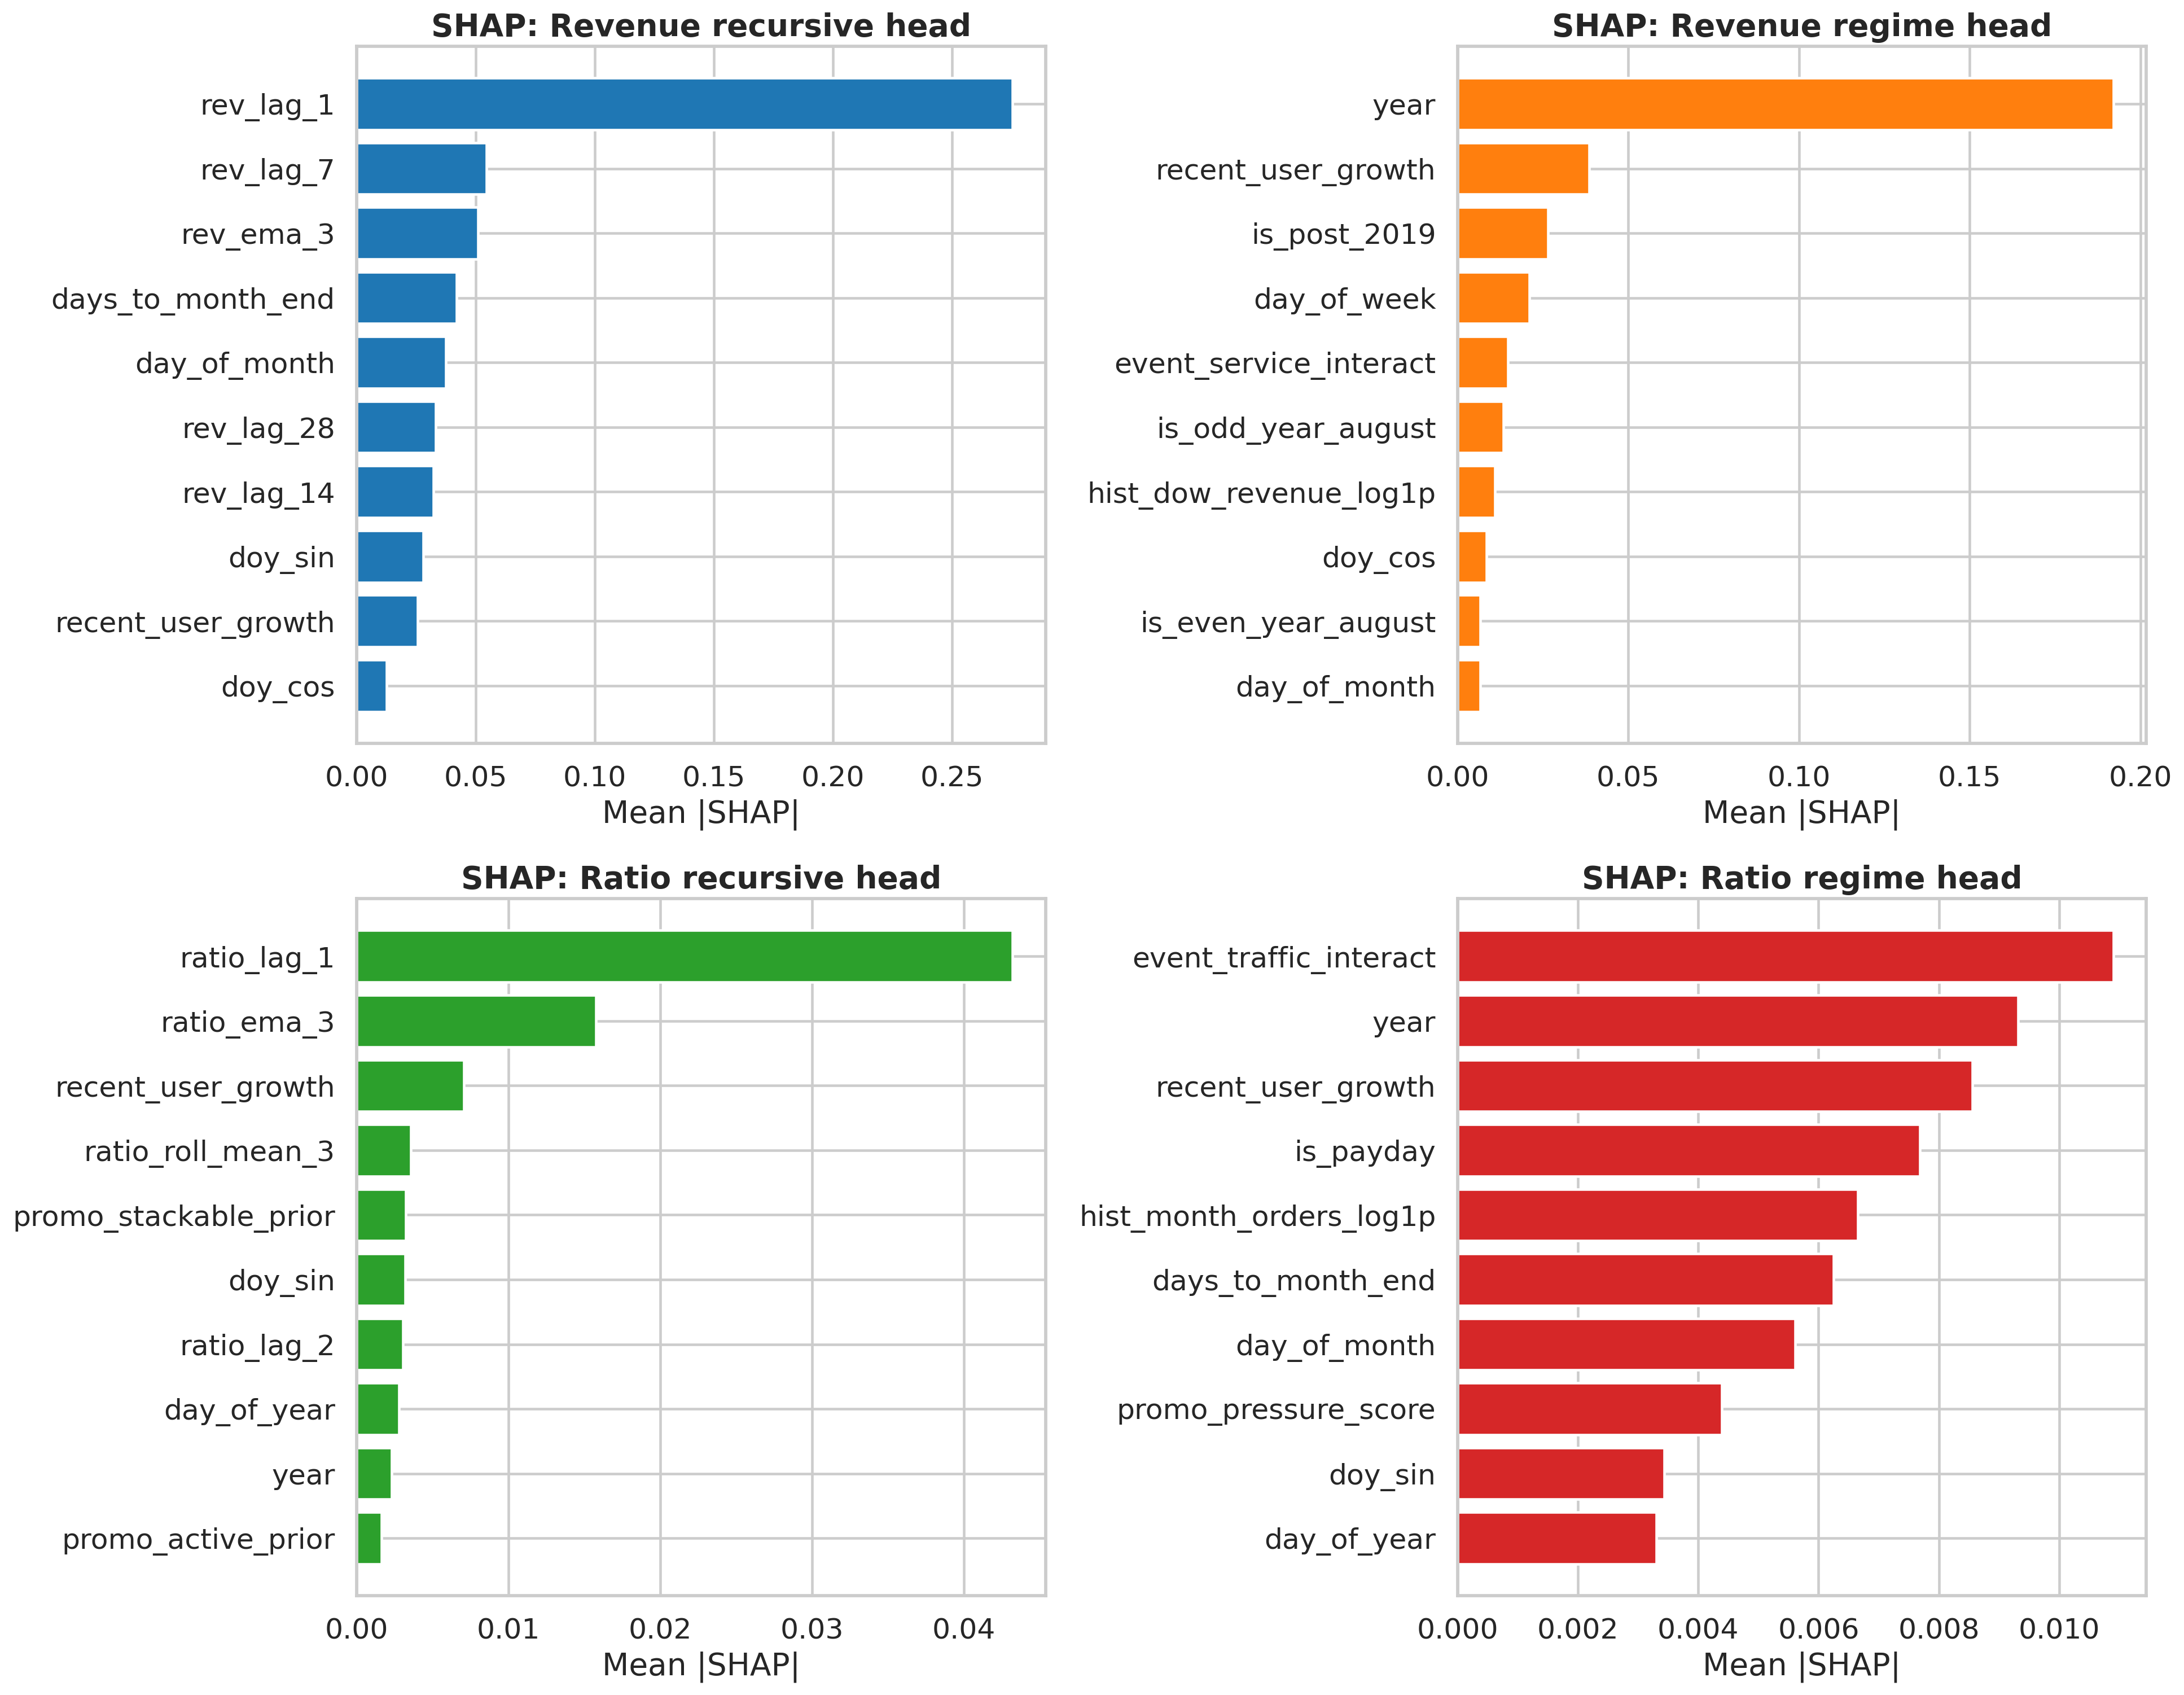
\includegraphics[width=\linewidth]{22_meta_horizon_shap_summary.png}
\captionof{figure}{Tổng hợp SHAP của các revenue specialist trong final line.}
\label{fig:appendix-shap}

\end{figure*}

\begin{figure*}[p]
\centering
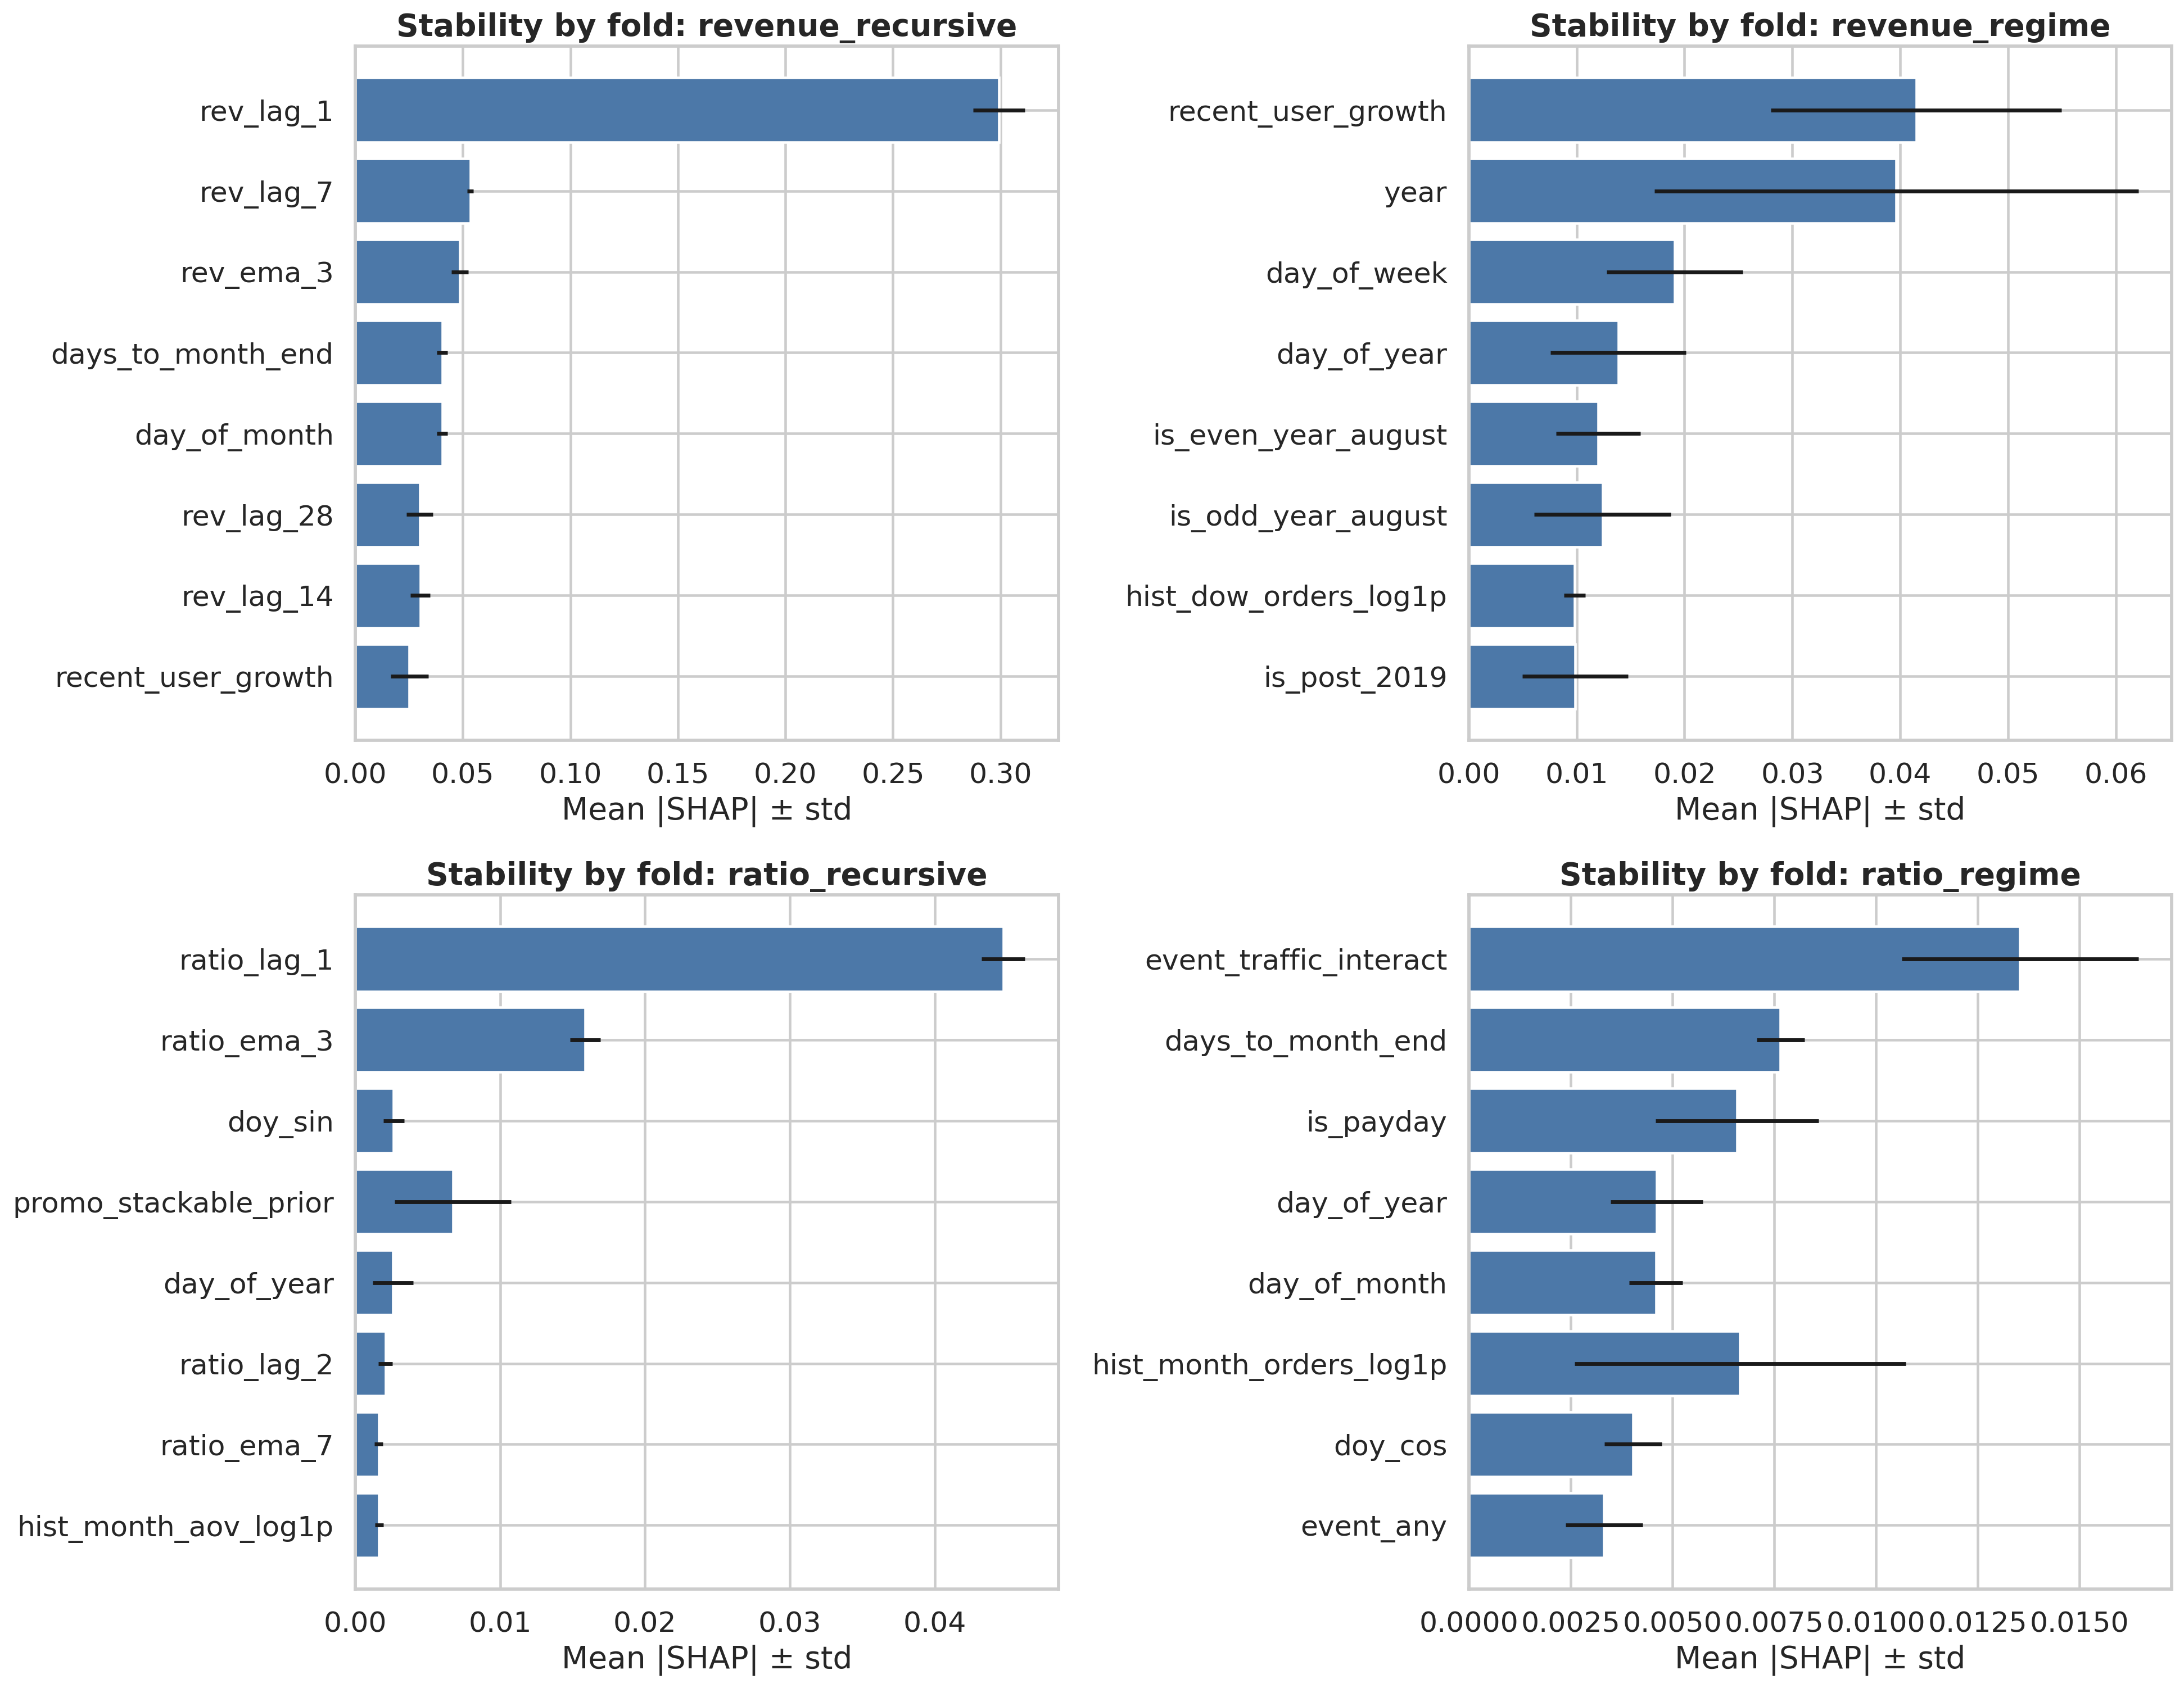
\includegraphics[width=\textwidth]{23_meta_horizon_feature_stability.png}
\caption{Độ ổn định của feature importance theo từng fold thời gian.}
\label{fig:appendix-stability}
\end{figure*}

\end{document}
